%% 可直接由仓库 paper/main.tex 通过 %% 可直接由仓库 paper/main.tex 通过 %% 可直接由仓库 paper/main.tex 通过 %% 可直接由仓库 paper/main.tex 通过 \input{sections/q1-quality-evaluation.tex} 引入。
%% 依照 paper/template/gmcmthesis.cls 的章节、公式、图形和 booktabs 表格规范编写。
\section{问题一：数据质量评价与基础评分}

\subsection{问题分析与总体框架}
本小问的目标是将抽样集与扩展集中的多源文本质量信号统一到同一评价尺度，形成可解释、可追溯的质量分数。评价对象包括抽样集 $A_1$、扩展集 $A_2$ 和扩展集 $A_3$ 的全部记录：$A_1$ 包含 $51{,}230$ 条记录，$A_2$ 包含 $17{,}523$ 条记录，$A_3$ 包含 $203{,}752$ 条记录。合并后先按记录指纹去重，得到 $261{,}086$ 条有效记录，去重前后删除 $11{,}419$ 条重复记录。模型流程为“全量合并与去重—指标方向统一—稳健归一化—CRITIC 客观赋权—加权距离 TOPSIS 评分—样本、领域和语料级聚合—抽样集对照”。

\begin{figure}[htbp]
  \centering
  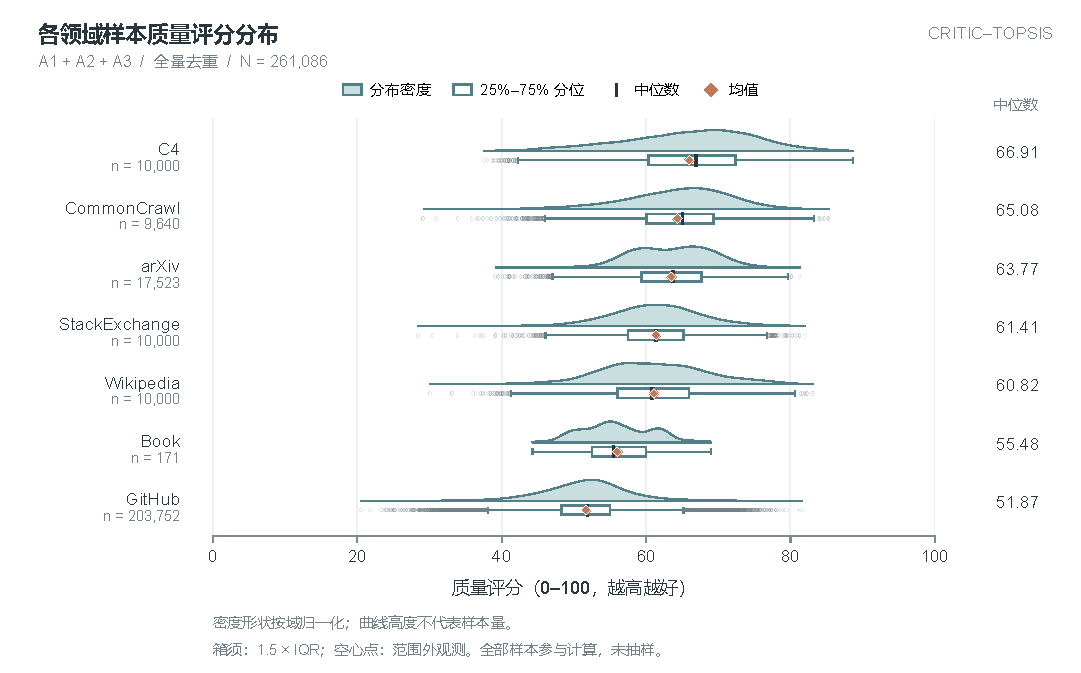
\includegraphics[width=\linewidth,height=0.42\textheight,keepaspectratio]{figures/q1-critic-topsis/nature-v1/figure01_domain_distribution_nature.pdf}
  \caption{领域质量分布图}
  \label{fig:q1-nature-01}
\end{figure}

\subsection{数据对象与预处理}
第 $i$ 条记录具有 16 维原始质量指标向量。指标覆盖语言形式、可读性、内容质量、教育性、事实性、知识覆盖与重复性等维度，其中句末标点率、cleanliness、no-ad、readability、fluency、unique words、QuRating education、writing、FineWeb education、factual、Books、Math 和 Wikipedia 为正向指标；无字母词比例、最高频二元词组占比和最高频三元词组占比为负向指标。负向指标较大时通常意味着文本更可能由符号、模板或高频短语主导，因此需要反向处理。
\formulaname{原始质量指标向量公式}
\begin{equation}
 \boldsymbol{x}_i=(x_{i1},\ldots,x_{i16}).
 \label{eq:q1-indicator-vector}
\end{equation}

正向与负向指标集合分别记为 $\mathcal P$、$\mathcal N$，两者互不相交且覆盖全部 16 个指标。方向统一后的指标定义如下。
\formulaname{指标方向统一公式}
\begin{equation}
 \widetilde{x}_{ij}=\begin{cases}
 x_{ij}, & j\in\mathcal{P},\\
 -x_{ij}, & j\in\mathcal{N}
 \end{cases}
 \label{eq:q1-direction-unification}
\end{equation}
随后使用方向统一值的 $A_1$ 拟合 $1\%$ 和 $99\%$ 分位点作为稳健边界；记边界为 $l_j$ 和 $u_j$，则统一为“越高越好”的稳健归一化形式。这里 $\operatorname{clip}(t,0,1)$ 表示将 $t$ 截断至 $[0,1]$。
\formulaname{稳健归一化公式}
\begin{equation}
 z_{ij}=\operatorname{clip}\left(\frac{\widetilde{x}_{ij}-l_j}{u_j-l_j},0,1\right).
 \label{eq:q1-robust-normalization}
\end{equation}
扩展集只使用 $A_1$ 的边界，不重新拟合分位点，从而保证 $A_1$、$A_2$ 和 $A_3$ 的分数具有可比性。归一化后检查缺失值、无穷值、越界值和重复指纹，并保留每条记录的来源集、领域标签和质量分数，供后续聚合与审计。

\begin{figure}[htbp]
  \centering
  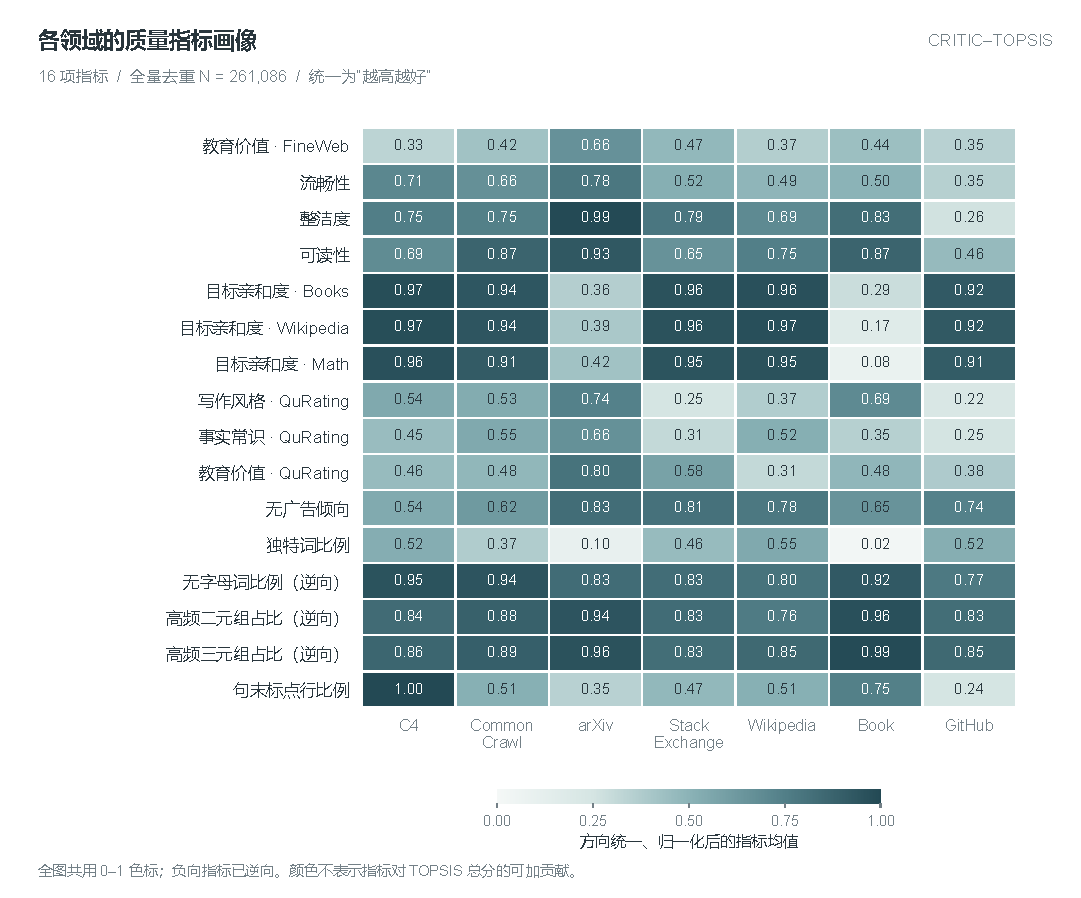
\includegraphics[width=\linewidth,height=0.42\textheight,keepaspectratio]{figures/q1-critic-topsis/nature-v1/figure02_indicator_heatmap_nature.pdf}
  \caption{领域质量指标画像图}
  \label{fig:q1-nature-02}
\end{figure}

\subsection{CRITIC 客观赋权}
为避免人为指定权重，采用 CRITIC 方法同时利用指标的离散程度和冲突程度。设归一化矩阵为 $Z$，其元素为 $z_{ij}$；第 $j$ 个指标的标准差为 $\sigma_j$，与第 $k$ 个指标的 Pearson 相关系数为 $r_{jk}$。
\formulaname{CRITIC 信息量公式}
\begin{equation}
 I_j=\sigma_j\sum_{k=1}^{16}(1-r_{jk}).
 \label{eq:q1-critic-information}
\end{equation}
\formulaname{CRITIC 权重公式}
\begin{equation}
 w_j=\frac{I_j}{\sum_{m=1}^{16}I_m}.
 \label{eq:q1-critic}
\end{equation}
其中，$\sigma_j$ 反映指标对样本的区分能力，$1-r_{jk}$ 反映该指标与其他指标的信息差异。由 $A_1$ 的拟合集计算权重并固定应用于 $A_1$ 留出集及 $A_2$、$A_3$，既防止扩展集的分布变化改变权重，又保证外推比较的可重复性。最终权重最高的指标为句末标点率（$8.9093\%$）、cleanliness（$8.0008\%$）和 no-ad（$7.7530\%$）；三个负向词组指标合计权重为 $16.5784\%$。

\begin{figure}[htbp]
  \centering
  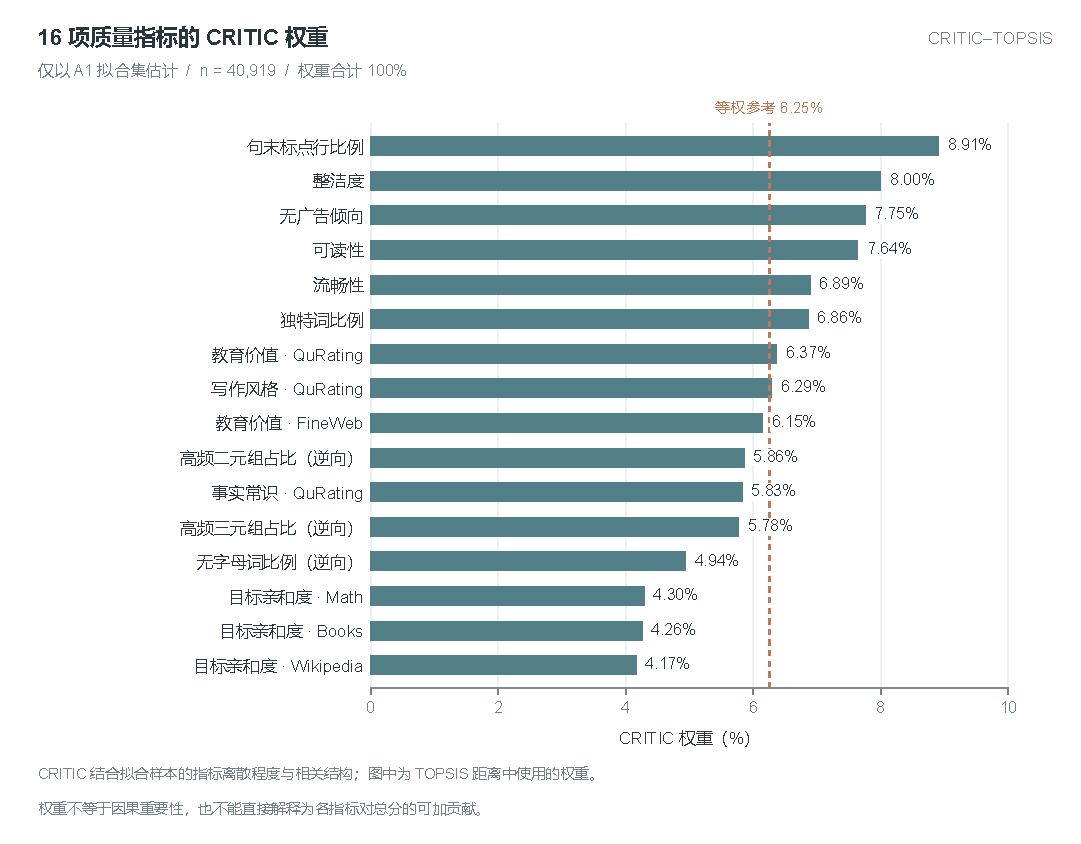
\includegraphics[width=\linewidth,height=0.42\textheight,keepaspectratio]{figures/q1-critic-topsis/nature-v1/figure05_critic_weights_nature.pdf}
  \caption{质量指标权重图}
  \label{fig:q1-nature-05}
\end{figure}

\subsection{加权距离 TOPSIS 评分}
以取值全为 1 的正向理想点 $\boldsymbol{z}^{+}$ 和取值全为 0 的负向理想点 $\boldsymbol{z}^{-}$ 为参照，计算第 $i$ 条记录到两类理想点的加权欧氏距离。
\formulaname{正理想点距离公式}
\begin{equation}
 D_i^{+}=\sqrt{\sum_{j=1}^{16}w_j(1-z_{ij})^2}.
 \label{eq:q1-topsis-positive-distance}
\end{equation}
\formulaname{负理想点距离公式}
\begin{equation}
 D_i^{-}=\sqrt{\sum_{j=1}^{16}w_jz_{ij}^2}.
 \label{eq:q1-topsis-distance}
\end{equation}
样本级质量分数定义如下，其取值在 $[0,100]$。
\formulaname{样本质量分数公式}
\begin{equation}
 Q_i=100\times\frac{D_i^{-}}{D_i^{+}+D_i^{-}}.
 \label{eq:q1-topsis-score}
\end{equation}
因此，$Q_i$ 越大表示该记录越接近理想高质量点。该分数回答的是“单条文本在 16 个统一方向质量信号下的综合质量水平”，而非某个单一指标的原始测量值。

\begin{figure}[htbp]
  \centering
  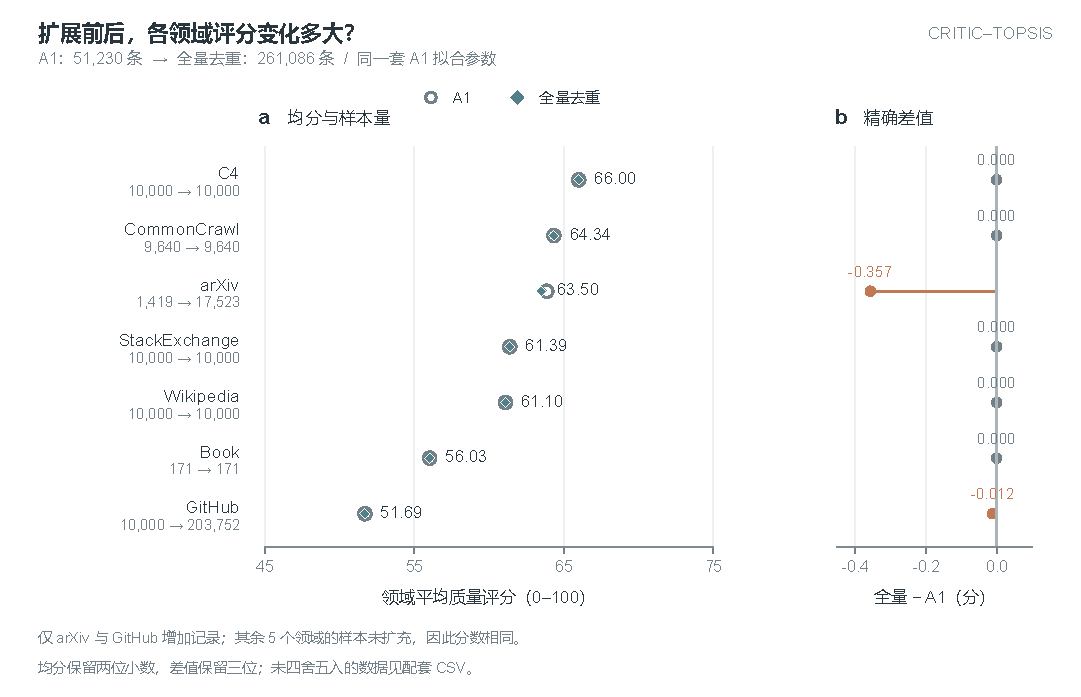
\includegraphics[width=\linewidth,height=0.42\textheight,keepaspectratio]{figures/q1-critic-topsis/nature-v1/figure03_A1_full_comparison_nature.pdf}
  \caption{领域均分对照图}
  \label{fig:q1-nature-03}
\end{figure}

\subsection{从样本级到领域级和语料级的聚合}
对领域 $g$ 的记录集合 $\mathcal{I}_g$，采用样本数加权的均值聚合。
\formulaname{领域质量均值公式}
\begin{equation}
 Q_g=\frac{1}{|\mathcal{I}_g|}\sum_{i\in\mathcal{I}_g}Q_i.
 \label{eq:q1-domain-aggregation}
\end{equation}
语料级分数同样由全体记录的样本均值给出。这种聚合保留了每条记录的等贡献原则，并能将域级差异与域规模分离：域均值反映质量，域记录数反映组成。若需降低极端值影响，可在附录中同时报告中位数和四分位距，但主结果使用均值以便与全量语料平均质量一致。
\formulaname{语料质量均值公式}
\begin{equation}
 Q_{\mathrm{corpus}}=\frac{1}{N}\sum_{i=1}^{N}Q_i.
 \label{eq:q1-corpus-aggregation}
\end{equation}

\begin{figure}[htbp]
  \centering
  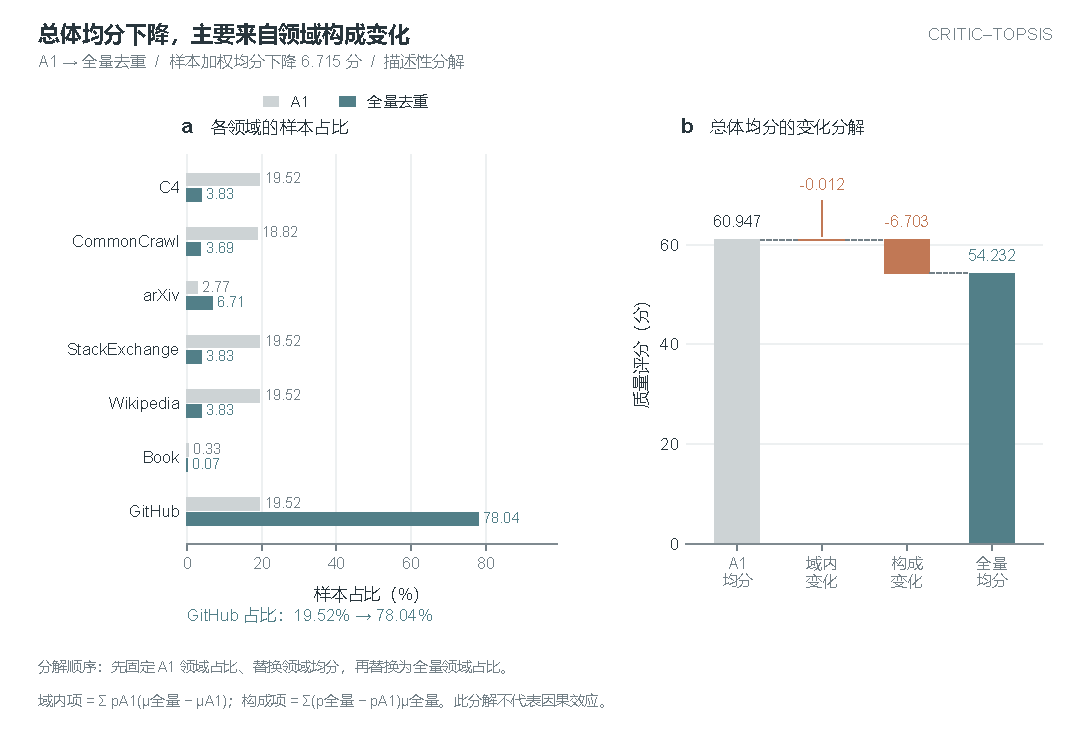
\includegraphics[width=\linewidth,height=0.42\textheight,keepaspectratio]{figures/q1-critic-topsis/nature-v1/figure04_composition_decomposition_nature.pdf}
  \caption{领域构成分解图}
  \label{fig:q1-nature-04}
\end{figure}

\subsection{全量结果与抽样集对照}
$A_1$ 语料级平均分为 $60.9471$，全量去重语料平均分为 $54.2323$，整体下降 $6.7149$ 分。按领域对照时，arxiv 从 $63.8624$ 变为 $63.5050$，下降 $0.3574$ 分；github 从 $51.7014$ 变为 $51.6893$，下降 $0.0121$ 分；book、c4、commoncrawl、stackexchange 和 wikipedia 的领域均值保持不变或仅发生四舍五入范围内的变化。由此可见，全量平均分下降主要来自领域组成变化，而不是各领域内部质量普遍恶化。GitHub 在 $A_1$ 中约占 $19.52\%$，在全量去重语料中约占 $78.04\%$，其较低的领域均值显著拉低了全量语料级分数。

\begin{table}[htbp]
  \centering
  \caption{$A_1$ 与全量去重语料的领域级质量分数对照}
  \label{tab:q1-domain-score}

  \renewcommand{\arraystretch}{1.15}
  \begin{tabular}{lrrrr}
    \toprule
    领域 & $A_1$ 均值 & 全量均值 & 变化 & 全量占比 \\
    \midrule
    arxiv & 63.8624 & 63.5050 & -0.3574 & 6.71\% \\
    book & 56.0325 & 56.0325 & 0.0000 & 0.07\% \\
    c4 & 66.0021 & 66.0021 & 0.0000 & 3.83\% \\
    commoncrawl & 64.3357 & 64.3357 & 0.0000 & 3.69\% \\
    github & 51.7014 & 51.6893 & -0.0121 & 78.04\% \\
    stackexchange & 61.3879 & 61.3879 & 0.0000 & 3.83\% \\
    wikipedia & 61.1009 & 61.1009 & 0.0000 & 3.83\% \\
    \addlinespace[0.5ex]
    语料级均值 & 60.9471 & 54.2323 & -6.7149 & 100.00\% \\
    \bottomrule
  \end{tabular}
\end{table}

\subsection{稳健性与适用边界}
将 CRITIC--TOPSIS 结果与等权加权、删除 DSIR 以及删除三个负向词组指标的敏感性方案比较。CRITIC 加权和等权结果的 Spearman 相关系数为 $0.9877$，CRITIC 结果与删除 DSIR 的结果相关系数为 $0.9860$，与删除三个负向指标的结果相关系数为 $0.9674$。在删除负向指标的方案中，平均名次变化为 $4.79$ 个百分点，约 $2.78\%$ 的记录名次变化超过 $20$ 个百分点，说明重复性指标虽不是唯一质量依据，但对尾部样本的排序具有实质影响。这里的敏感性分析用于检查第一小问质量评分对建模选择的稳定性；它不等同于问题一后续小问中对指标冲突的独立量化。

\begin{figure}[htbp]
  \centering
  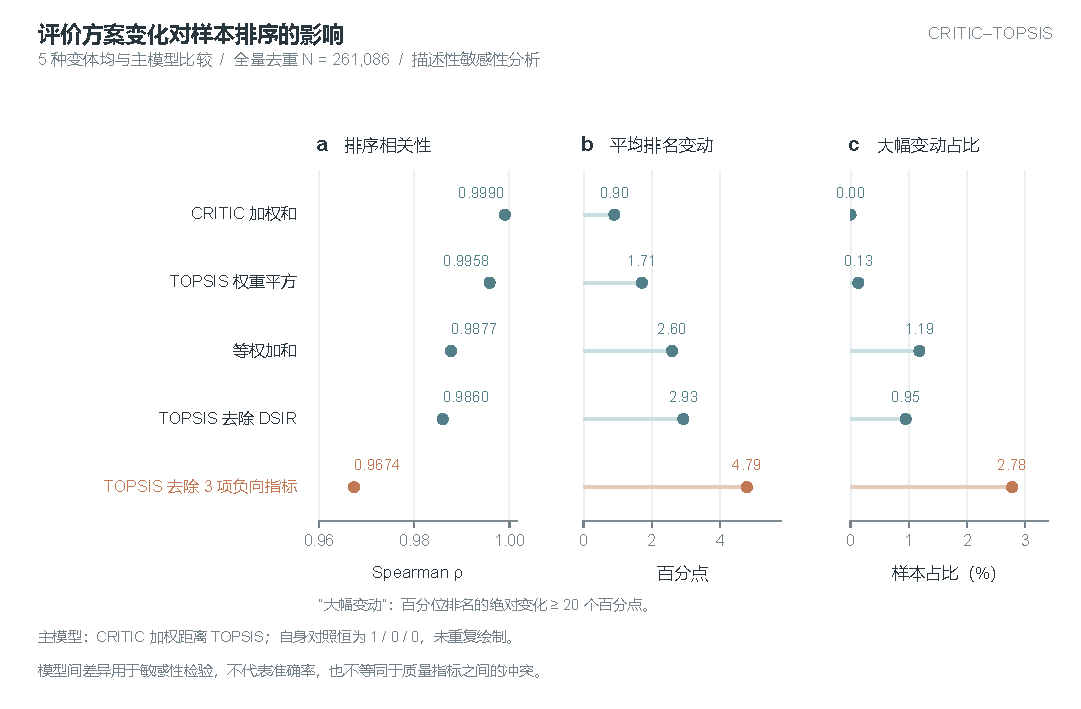
\includegraphics[width=\linewidth,height=0.42\textheight,keepaspectratio]{figures/q1-critic-topsis/nature-v1/figure06_model_sensitivity_nature.pdf}
  \caption{评分排序敏感性图}
  \label{fig:q1-nature-06}
\end{figure}

\subsection{小结}
本小问形成了一个可复算的全量质量评价链条：以 $A_1$ 的稳健边界和 CRITIC 权重建立统一标尺，以加权距离 TOPSIS 输出样本级质量分数，再按记录均值聚合为领域级和语料级分数。结果表明，$A_1$ 与扩展后的全量语料在领域内部质量上总体稳定，语料级平均分的主要变化由领域配比改变所致。该结论为后续质量冲突识别和数据配比优化提供可追溯的基线。
 引入。
%% 依照 paper/template/gmcmthesis.cls 的章节、公式、图形和 booktabs 表格规范编写。
\section{问题一：数据质量评价与基础评分}

\subsection{问题分析与总体框架}
本小问的目标是将抽样集与扩展集中的多源文本质量信号统一到同一评价尺度，形成可解释、可追溯的质量分数。评价对象包括抽样集 $A_1$、扩展集 $A_2$ 和扩展集 $A_3$ 的全部记录：$A_1$ 包含 $51{,}230$ 条记录，$A_2$ 包含 $17{,}523$ 条记录，$A_3$ 包含 $203{,}752$ 条记录。合并后先按记录指纹去重，得到 $261{,}086$ 条有效记录，去重前后删除 $11{,}419$ 条重复记录。模型流程为“全量合并与去重—指标方向统一—稳健归一化—CRITIC 客观赋权—加权距离 TOPSIS 评分—样本、领域和语料级聚合—抽样集对照”。

\begin{figure}[htbp]
  \centering
  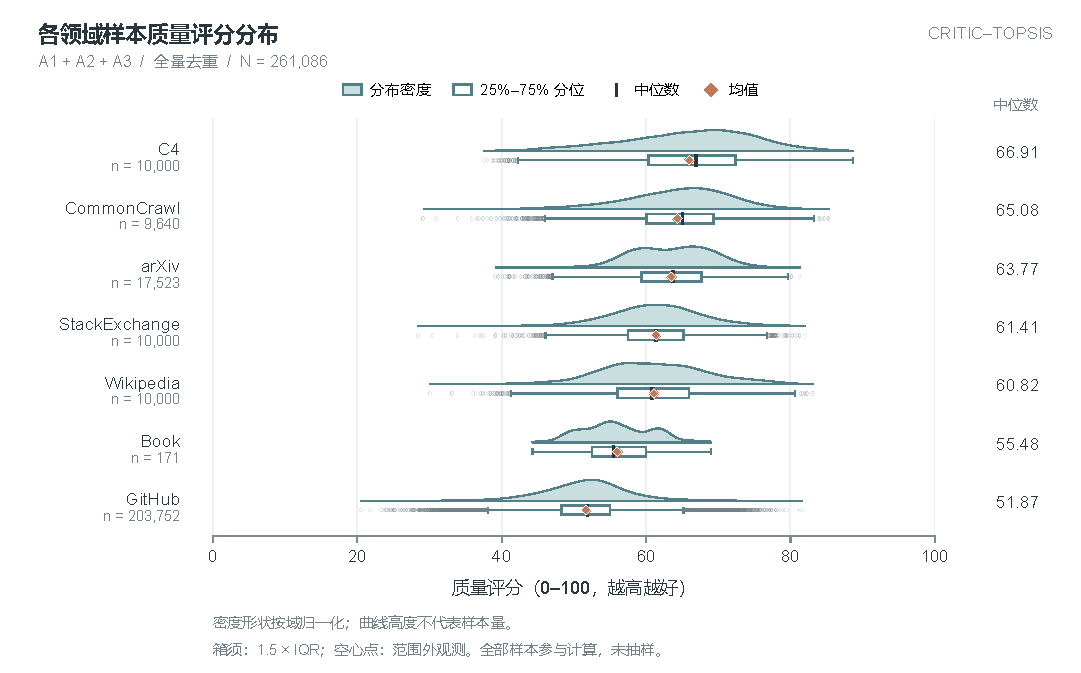
\includegraphics[width=\linewidth,height=0.42\textheight,keepaspectratio]{figures/q1-critic-topsis/nature-v1/figure01_domain_distribution_nature.pdf}
  \caption{领域质量分布图}
  \label{fig:q1-nature-01}
\end{figure}

\subsection{数据对象与预处理}
第 $i$ 条记录具有 16 维原始质量指标向量。指标覆盖语言形式、可读性、内容质量、教育性、事实性、知识覆盖与重复性等维度，其中句末标点率、cleanliness、no-ad、readability、fluency、unique words、QuRating education、writing、FineWeb education、factual、Books、Math 和 Wikipedia 为正向指标；无字母词比例、最高频二元词组占比和最高频三元词组占比为负向指标。负向指标较大时通常意味着文本更可能由符号、模板或高频短语主导，因此需要反向处理。
\formulaname{原始质量指标向量公式}
\begin{equation}
 \boldsymbol{x}_i=(x_{i1},\ldots,x_{i16}).
 \label{eq:q1-indicator-vector}
\end{equation}

正向与负向指标集合分别记为 $\mathcal P$、$\mathcal N$，两者互不相交且覆盖全部 16 个指标。方向统一后的指标定义如下。
\formulaname{指标方向统一公式}
\begin{equation}
 \widetilde{x}_{ij}=\begin{cases}
 x_{ij}, & j\in\mathcal{P},\\
 -x_{ij}, & j\in\mathcal{N}
 \end{cases}
 \label{eq:q1-direction-unification}
\end{equation}
随后使用方向统一值的 $A_1$ 拟合 $1\%$ 和 $99\%$ 分位点作为稳健边界；记边界为 $l_j$ 和 $u_j$，则统一为“越高越好”的稳健归一化形式。这里 $\operatorname{clip}(t,0,1)$ 表示将 $t$ 截断至 $[0,1]$。
\formulaname{稳健归一化公式}
\begin{equation}
 z_{ij}=\operatorname{clip}\left(\frac{\widetilde{x}_{ij}-l_j}{u_j-l_j},0,1\right).
 \label{eq:q1-robust-normalization}
\end{equation}
扩展集只使用 $A_1$ 的边界，不重新拟合分位点，从而保证 $A_1$、$A_2$ 和 $A_3$ 的分数具有可比性。归一化后检查缺失值、无穷值、越界值和重复指纹，并保留每条记录的来源集、领域标签和质量分数，供后续聚合与审计。

\begin{figure}[htbp]
  \centering
  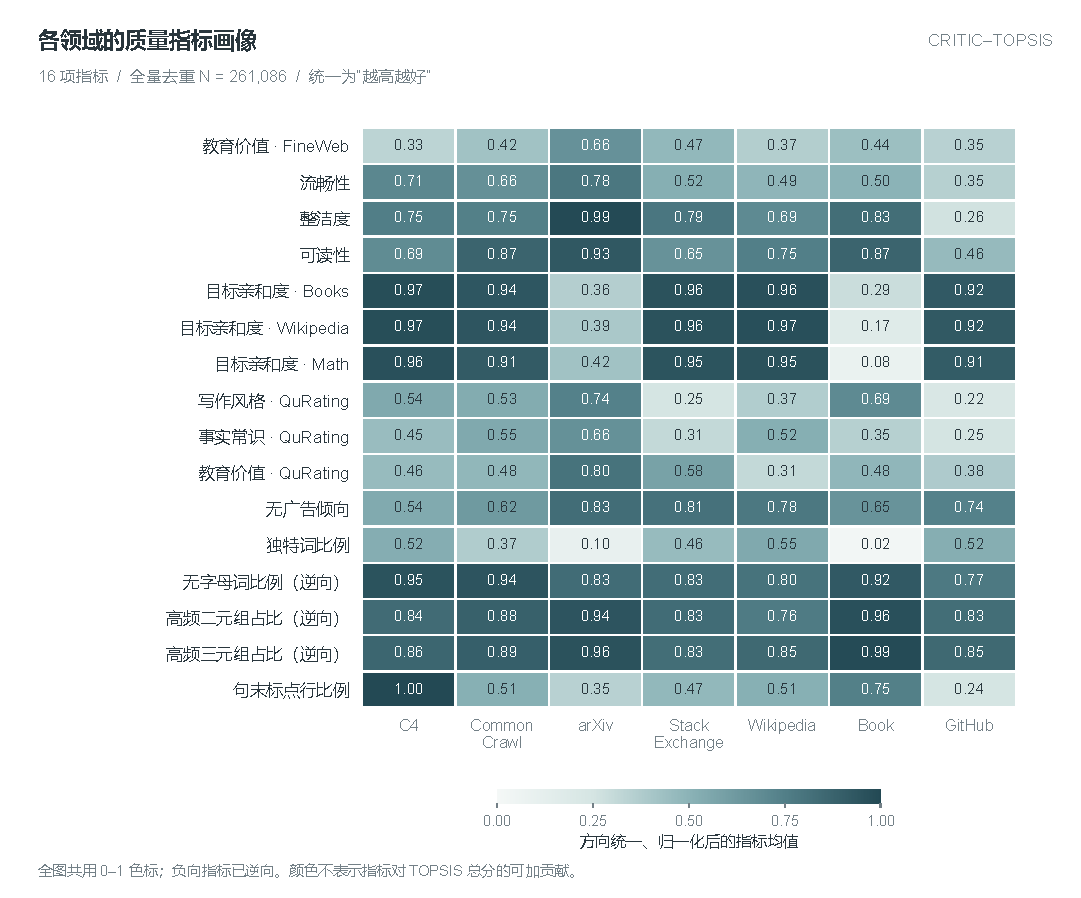
\includegraphics[width=\linewidth,height=0.42\textheight,keepaspectratio]{figures/q1-critic-topsis/nature-v1/figure02_indicator_heatmap_nature.pdf}
  \caption{领域质量指标画像图}
  \label{fig:q1-nature-02}
\end{figure}

\subsection{CRITIC 客观赋权}
为避免人为指定权重，采用 CRITIC 方法同时利用指标的离散程度和冲突程度。设归一化矩阵为 $Z$，其元素为 $z_{ij}$；第 $j$ 个指标的标准差为 $\sigma_j$，与第 $k$ 个指标的 Pearson 相关系数为 $r_{jk}$。
\formulaname{CRITIC 信息量公式}
\begin{equation}
 I_j=\sigma_j\sum_{k=1}^{16}(1-r_{jk}).
 \label{eq:q1-critic-information}
\end{equation}
\formulaname{CRITIC 权重公式}
\begin{equation}
 w_j=\frac{I_j}{\sum_{m=1}^{16}I_m}.
 \label{eq:q1-critic}
\end{equation}
其中，$\sigma_j$ 反映指标对样本的区分能力，$1-r_{jk}$ 反映该指标与其他指标的信息差异。由 $A_1$ 的拟合集计算权重并固定应用于 $A_1$ 留出集及 $A_2$、$A_3$，既防止扩展集的分布变化改变权重，又保证外推比较的可重复性。最终权重最高的指标为句末标点率（$8.9093\%$）、cleanliness（$8.0008\%$）和 no-ad（$7.7530\%$）；三个负向词组指标合计权重为 $16.5784\%$。

\begin{figure}[htbp]
  \centering
  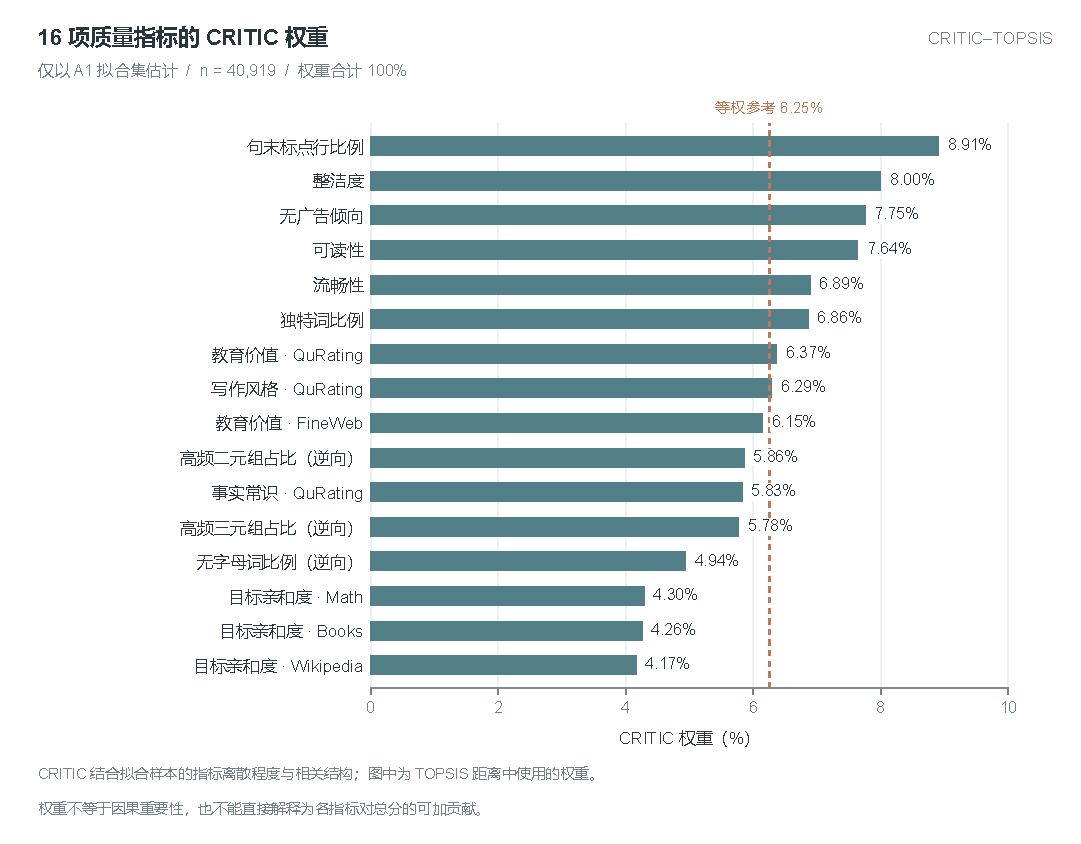
\includegraphics[width=\linewidth,height=0.42\textheight,keepaspectratio]{figures/q1-critic-topsis/nature-v1/figure05_critic_weights_nature.pdf}
  \caption{质量指标权重图}
  \label{fig:q1-nature-05}
\end{figure}

\subsection{加权距离 TOPSIS 评分}
以取值全为 1 的正向理想点 $\boldsymbol{z}^{+}$ 和取值全为 0 的负向理想点 $\boldsymbol{z}^{-}$ 为参照，计算第 $i$ 条记录到两类理想点的加权欧氏距离。
\formulaname{正理想点距离公式}
\begin{equation}
 D_i^{+}=\sqrt{\sum_{j=1}^{16}w_j(1-z_{ij})^2}.
 \label{eq:q1-topsis-positive-distance}
\end{equation}
\formulaname{负理想点距离公式}
\begin{equation}
 D_i^{-}=\sqrt{\sum_{j=1}^{16}w_jz_{ij}^2}.
 \label{eq:q1-topsis-distance}
\end{equation}
样本级质量分数定义如下，其取值在 $[0,100]$。
\formulaname{样本质量分数公式}
\begin{equation}
 Q_i=100\times\frac{D_i^{-}}{D_i^{+}+D_i^{-}}.
 \label{eq:q1-topsis-score}
\end{equation}
因此，$Q_i$ 越大表示该记录越接近理想高质量点。该分数回答的是“单条文本在 16 个统一方向质量信号下的综合质量水平”，而非某个单一指标的原始测量值。

\begin{figure}[htbp]
  \centering
  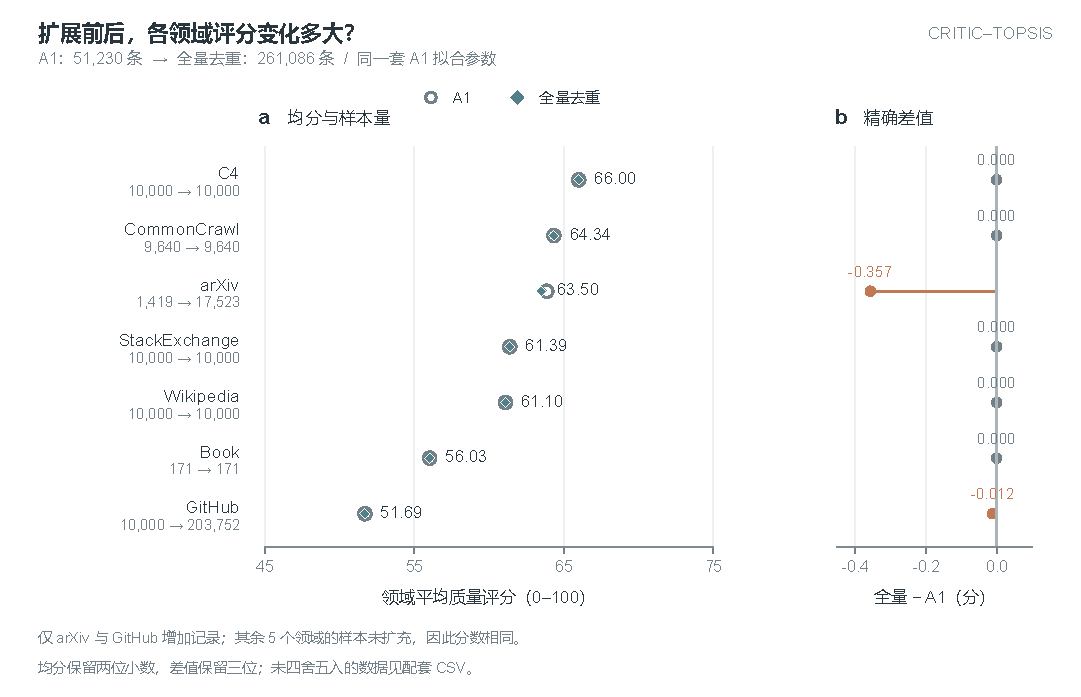
\includegraphics[width=\linewidth,height=0.42\textheight,keepaspectratio]{figures/q1-critic-topsis/nature-v1/figure03_A1_full_comparison_nature.pdf}
  \caption{领域均分对照图}
  \label{fig:q1-nature-03}
\end{figure}

\subsection{从样本级到领域级和语料级的聚合}
对领域 $g$ 的记录集合 $\mathcal{I}_g$，采用样本数加权的均值聚合。
\formulaname{领域质量均值公式}
\begin{equation}
 Q_g=\frac{1}{|\mathcal{I}_g|}\sum_{i\in\mathcal{I}_g}Q_i.
 \label{eq:q1-domain-aggregation}
\end{equation}
语料级分数同样由全体记录的样本均值给出。这种聚合保留了每条记录的等贡献原则，并能将域级差异与域规模分离：域均值反映质量，域记录数反映组成。若需降低极端值影响，可在附录中同时报告中位数和四分位距，但主结果使用均值以便与全量语料平均质量一致。
\formulaname{语料质量均值公式}
\begin{equation}
 Q_{\mathrm{corpus}}=\frac{1}{N}\sum_{i=1}^{N}Q_i.
 \label{eq:q1-corpus-aggregation}
\end{equation}

\begin{figure}[htbp]
  \centering
  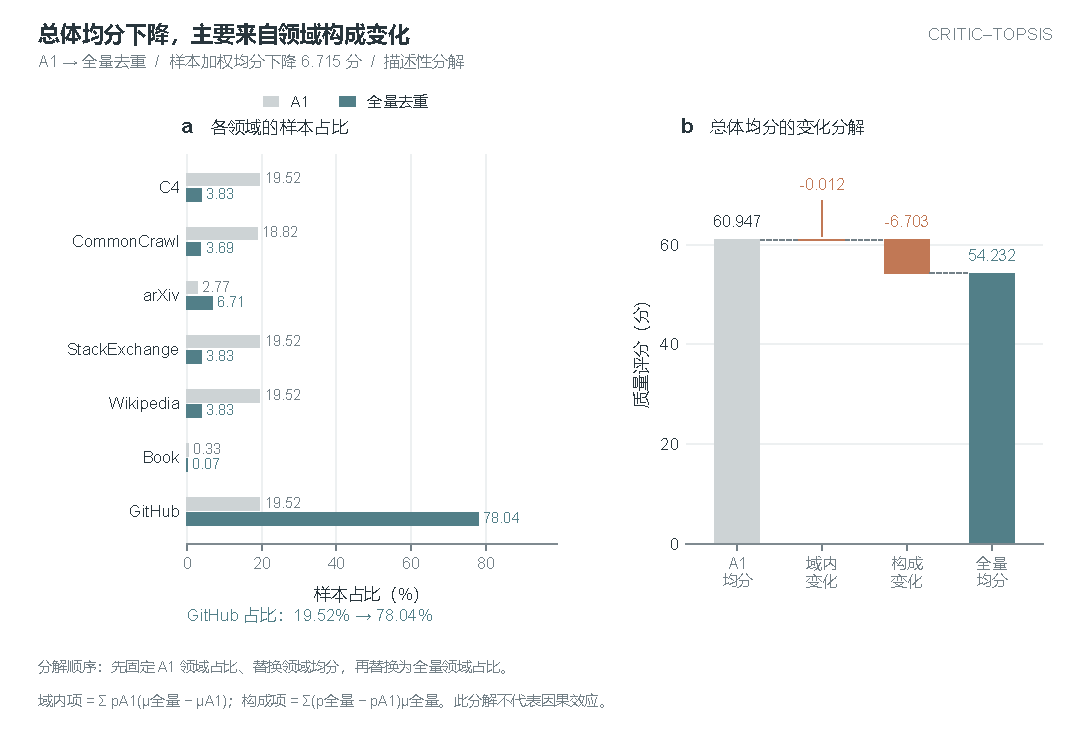
\includegraphics[width=\linewidth,height=0.42\textheight,keepaspectratio]{figures/q1-critic-topsis/nature-v1/figure04_composition_decomposition_nature.pdf}
  \caption{领域构成分解图}
  \label{fig:q1-nature-04}
\end{figure}

\subsection{全量结果与抽样集对照}
$A_1$ 语料级平均分为 $60.9471$，全量去重语料平均分为 $54.2323$，整体下降 $6.7149$ 分。按领域对照时，arxiv 从 $63.8624$ 变为 $63.5050$，下降 $0.3574$ 分；github 从 $51.7014$ 变为 $51.6893$，下降 $0.0121$ 分；book、c4、commoncrawl、stackexchange 和 wikipedia 的领域均值保持不变或仅发生四舍五入范围内的变化。由此可见，全量平均分下降主要来自领域组成变化，而不是各领域内部质量普遍恶化。GitHub 在 $A_1$ 中约占 $19.52\%$，在全量去重语料中约占 $78.04\%$，其较低的领域均值显著拉低了全量语料级分数。

\begin{table}[htbp]
  \centering
  \caption{$A_1$ 与全量去重语料的领域级质量分数对照}
  \label{tab:q1-domain-score}

  \renewcommand{\arraystretch}{1.15}
  \begin{tabular}{lrrrr}
    \toprule
    领域 & $A_1$ 均值 & 全量均值 & 变化 & 全量占比 \\
    \midrule
    arxiv & 63.8624 & 63.5050 & -0.3574 & 6.71\% \\
    book & 56.0325 & 56.0325 & 0.0000 & 0.07\% \\
    c4 & 66.0021 & 66.0021 & 0.0000 & 3.83\% \\
    commoncrawl & 64.3357 & 64.3357 & 0.0000 & 3.69\% \\
    github & 51.7014 & 51.6893 & -0.0121 & 78.04\% \\
    stackexchange & 61.3879 & 61.3879 & 0.0000 & 3.83\% \\
    wikipedia & 61.1009 & 61.1009 & 0.0000 & 3.83\% \\
    \addlinespace[0.5ex]
    语料级均值 & 60.9471 & 54.2323 & -6.7149 & 100.00\% \\
    \bottomrule
  \end{tabular}
\end{table}

\subsection{稳健性与适用边界}
将 CRITIC--TOPSIS 结果与等权加权、删除 DSIR 以及删除三个负向词组指标的敏感性方案比较。CRITIC 加权和等权结果的 Spearman 相关系数为 $0.9877$，CRITIC 结果与删除 DSIR 的结果相关系数为 $0.9860$，与删除三个负向指标的结果相关系数为 $0.9674$。在删除负向指标的方案中，平均名次变化为 $4.79$ 个百分点，约 $2.78\%$ 的记录名次变化超过 $20$ 个百分点，说明重复性指标虽不是唯一质量依据，但对尾部样本的排序具有实质影响。这里的敏感性分析用于检查第一小问质量评分对建模选择的稳定性；它不等同于问题一后续小问中对指标冲突的独立量化。

\begin{figure}[htbp]
  \centering
  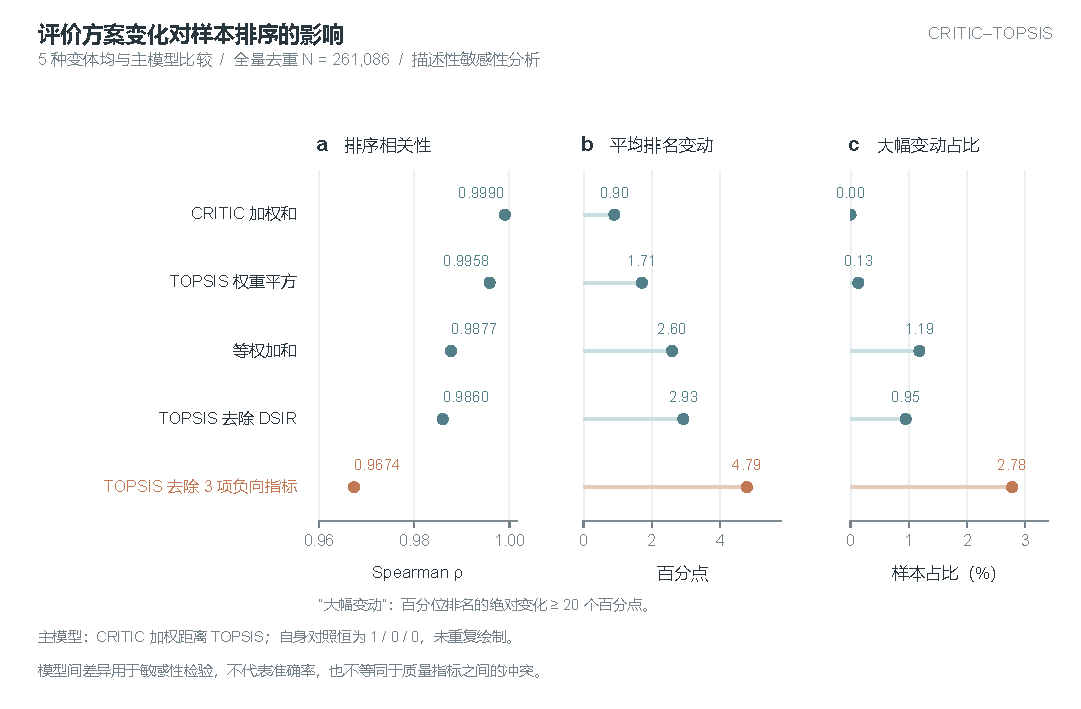
\includegraphics[width=\linewidth,height=0.42\textheight,keepaspectratio]{figures/q1-critic-topsis/nature-v1/figure06_model_sensitivity_nature.pdf}
  \caption{评分排序敏感性图}
  \label{fig:q1-nature-06}
\end{figure}

\subsection{小结}
本小问形成了一个可复算的全量质量评价链条：以 $A_1$ 的稳健边界和 CRITIC 权重建立统一标尺，以加权距离 TOPSIS 输出样本级质量分数，再按记录均值聚合为领域级和语料级分数。结果表明，$A_1$ 与扩展后的全量语料在领域内部质量上总体稳定，语料级平均分的主要变化由领域配比改变所致。该结论为后续质量冲突识别和数据配比优化提供可追溯的基线。
 引入。
%% 依照 paper/template/gmcmthesis.cls 的章节、公式、图形和 booktabs 表格规范编写。
\section{问题一：数据质量评价与基础评分}

\subsection{问题分析与总体框架}
本小问的目标是将抽样集与扩展集中的多源文本质量信号统一到同一评价尺度，形成可解释、可追溯的质量分数。评价对象包括抽样集 $A_1$、扩展集 $A_2$ 和扩展集 $A_3$ 的全部记录：$A_1$ 包含 $51{,}230$ 条记录，$A_2$ 包含 $17{,}523$ 条记录，$A_3$ 包含 $203{,}752$ 条记录。合并后先按记录指纹去重，得到 $261{,}086$ 条有效记录，去重前后删除 $11{,}419$ 条重复记录。模型流程为“全量合并与去重—指标方向统一—稳健归一化—CRITIC 客观赋权—加权距离 TOPSIS 评分—样本、领域和语料级聚合—抽样集对照”。

\begin{figure}[htbp]
  \centering
  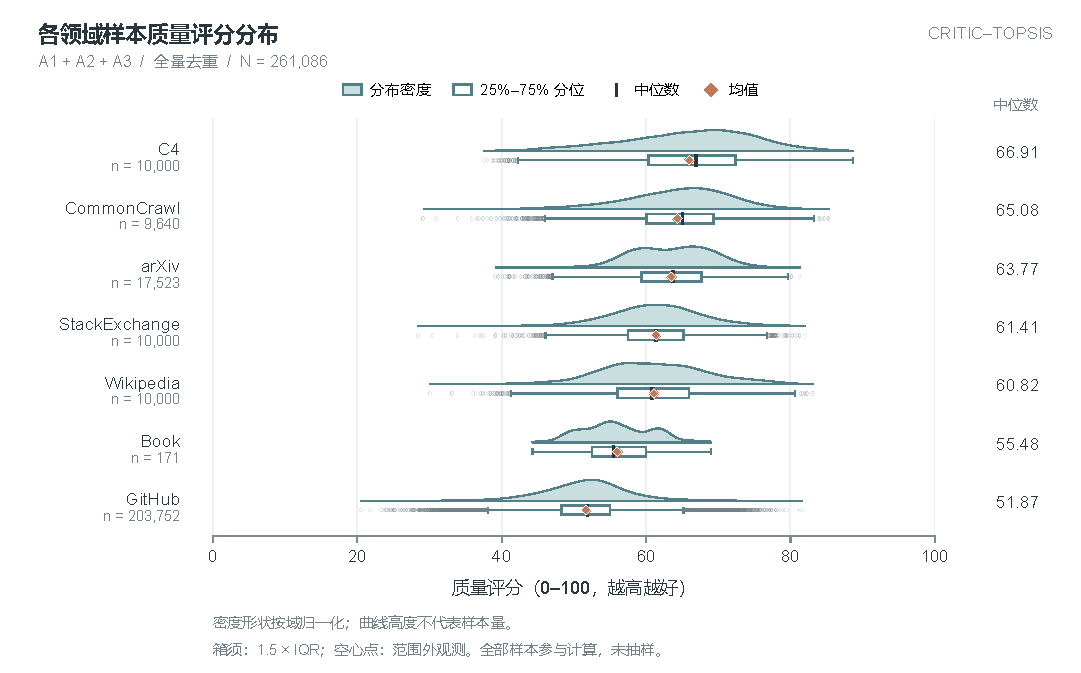
\includegraphics[width=\linewidth,height=0.42\textheight,keepaspectratio]{figures/q1-critic-topsis/nature-v1/figure01_domain_distribution_nature.pdf}
  \caption{领域质量分布图}
  \label{fig:q1-nature-01}
\end{figure}

\subsection{数据对象与预处理}
第 $i$ 条记录具有 16 维原始质量指标向量。指标覆盖语言形式、可读性、内容质量、教育性、事实性、知识覆盖与重复性等维度，其中句末标点率、cleanliness、no-ad、readability、fluency、unique words、QuRating education、writing、FineWeb education、factual、Books、Math 和 Wikipedia 为正向指标；无字母词比例、最高频二元词组占比和最高频三元词组占比为负向指标。负向指标较大时通常意味着文本更可能由符号、模板或高频短语主导，因此需要反向处理。
\formulaname{原始质量指标向量公式}
\begin{equation}
 \boldsymbol{x}_i=(x_{i1},\ldots,x_{i16}).
 \label{eq:q1-indicator-vector}
\end{equation}

正向与负向指标集合分别记为 $\mathcal P$、$\mathcal N$，两者互不相交且覆盖全部 16 个指标。方向统一后的指标定义如下。
\formulaname{指标方向统一公式}
\begin{equation}
 \widetilde{x}_{ij}=\begin{cases}
 x_{ij}, & j\in\mathcal{P},\\
 -x_{ij}, & j\in\mathcal{N}
 \end{cases}
 \label{eq:q1-direction-unification}
\end{equation}
随后使用方向统一值的 $A_1$ 拟合 $1\%$ 和 $99\%$ 分位点作为稳健边界；记边界为 $l_j$ 和 $u_j$，则统一为“越高越好”的稳健归一化形式。这里 $\operatorname{clip}(t,0,1)$ 表示将 $t$ 截断至 $[0,1]$。
\formulaname{稳健归一化公式}
\begin{equation}
 z_{ij}=\operatorname{clip}\left(\frac{\widetilde{x}_{ij}-l_j}{u_j-l_j},0,1\right).
 \label{eq:q1-robust-normalization}
\end{equation}
扩展集只使用 $A_1$ 的边界，不重新拟合分位点，从而保证 $A_1$、$A_2$ 和 $A_3$ 的分数具有可比性。归一化后检查缺失值、无穷值、越界值和重复指纹，并保留每条记录的来源集、领域标签和质量分数，供后续聚合与审计。

\begin{figure}[htbp]
  \centering
  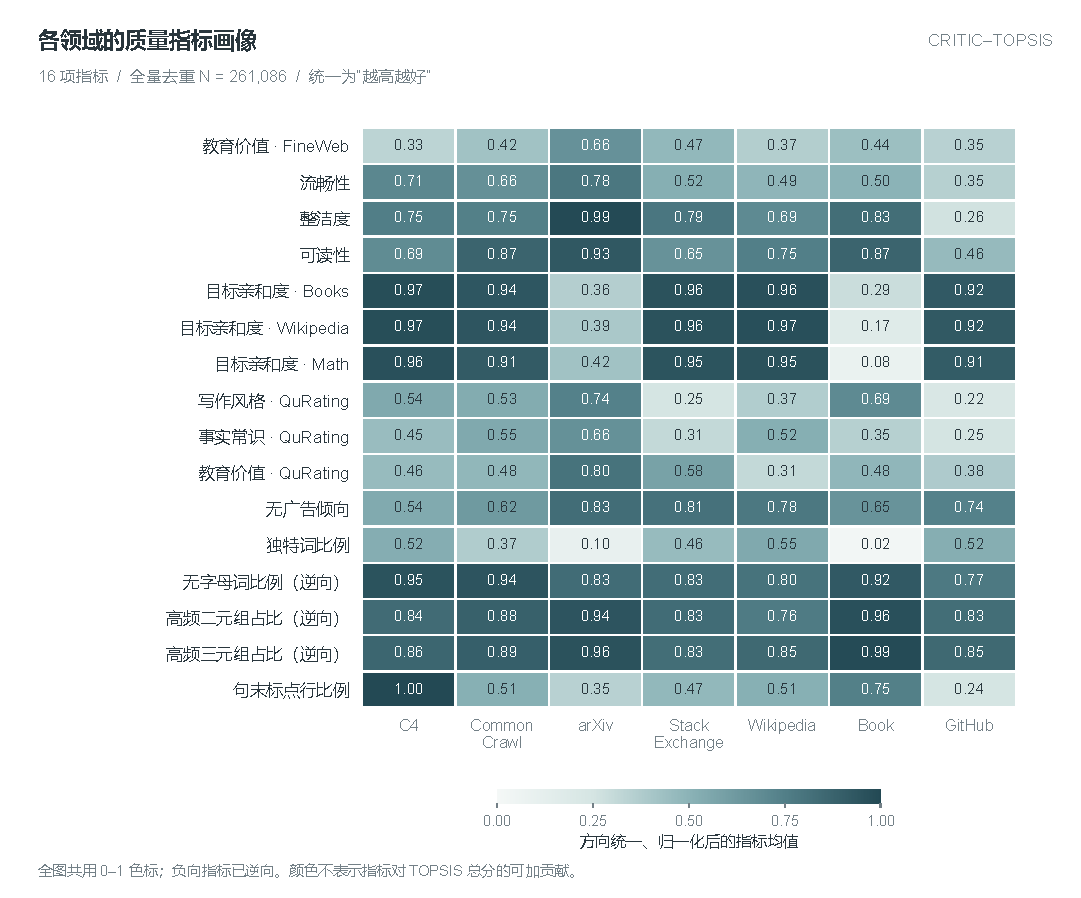
\includegraphics[width=\linewidth,height=0.42\textheight,keepaspectratio]{figures/q1-critic-topsis/nature-v1/figure02_indicator_heatmap_nature.pdf}
  \caption{领域质量指标画像图}
  \label{fig:q1-nature-02}
\end{figure}

\subsection{CRITIC 客观赋权}
为避免人为指定权重，采用 CRITIC 方法同时利用指标的离散程度和冲突程度。设归一化矩阵为 $Z$，其元素为 $z_{ij}$；第 $j$ 个指标的标准差为 $\sigma_j$，与第 $k$ 个指标的 Pearson 相关系数为 $r_{jk}$。
\formulaname{CRITIC 信息量公式}
\begin{equation}
 I_j=\sigma_j\sum_{k=1}^{16}(1-r_{jk}).
 \label{eq:q1-critic-information}
\end{equation}
\formulaname{CRITIC 权重公式}
\begin{equation}
 w_j=\frac{I_j}{\sum_{m=1}^{16}I_m}.
 \label{eq:q1-critic}
\end{equation}
其中，$\sigma_j$ 反映指标对样本的区分能力，$1-r_{jk}$ 反映该指标与其他指标的信息差异。由 $A_1$ 的拟合集计算权重并固定应用于 $A_1$ 留出集及 $A_2$、$A_3$，既防止扩展集的分布变化改变权重，又保证外推比较的可重复性。最终权重最高的指标为句末标点率（$8.9093\%$）、cleanliness（$8.0008\%$）和 no-ad（$7.7530\%$）；三个负向词组指标合计权重为 $16.5784\%$。

\begin{figure}[htbp]
  \centering
  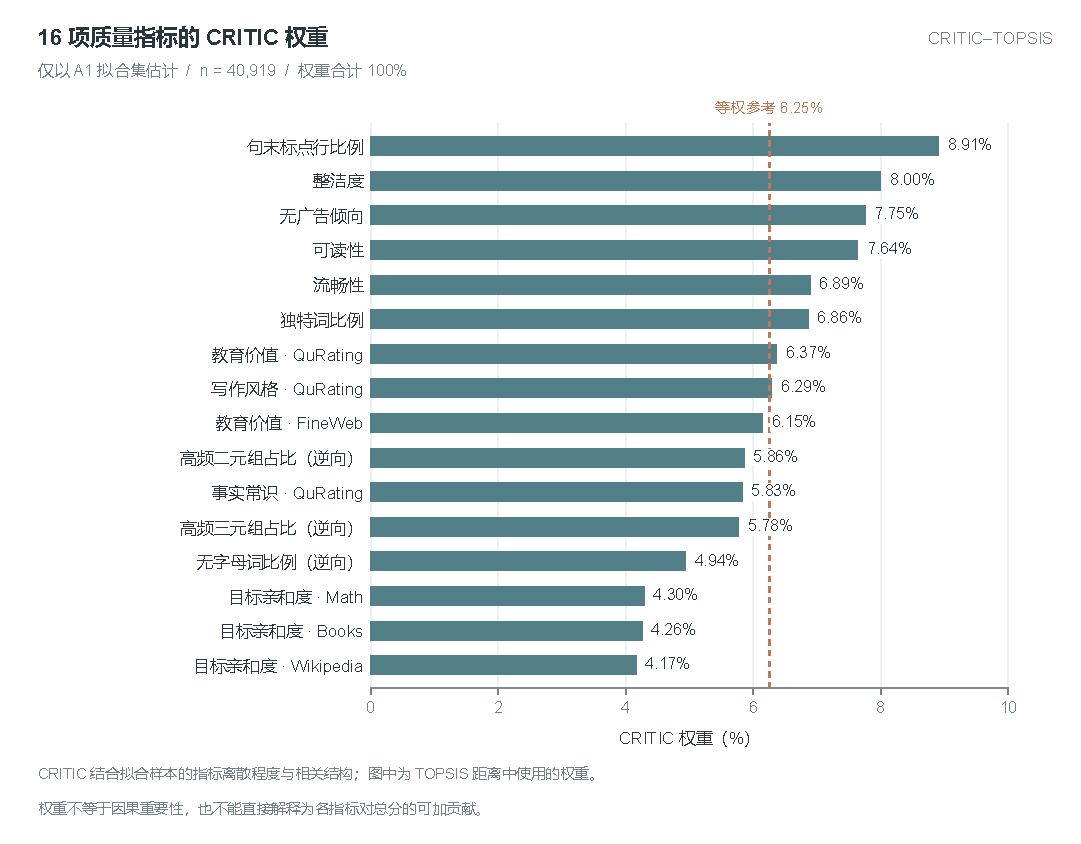
\includegraphics[width=\linewidth,height=0.42\textheight,keepaspectratio]{figures/q1-critic-topsis/nature-v1/figure05_critic_weights_nature.pdf}
  \caption{质量指标权重图}
  \label{fig:q1-nature-05}
\end{figure}

\subsection{加权距离 TOPSIS 评分}
以取值全为 1 的正向理想点 $\boldsymbol{z}^{+}$ 和取值全为 0 的负向理想点 $\boldsymbol{z}^{-}$ 为参照，计算第 $i$ 条记录到两类理想点的加权欧氏距离。
\formulaname{正理想点距离公式}
\begin{equation}
 D_i^{+}=\sqrt{\sum_{j=1}^{16}w_j(1-z_{ij})^2}.
 \label{eq:q1-topsis-positive-distance}
\end{equation}
\formulaname{负理想点距离公式}
\begin{equation}
 D_i^{-}=\sqrt{\sum_{j=1}^{16}w_jz_{ij}^2}.
 \label{eq:q1-topsis-distance}
\end{equation}
样本级质量分数定义如下，其取值在 $[0,100]$。
\formulaname{样本质量分数公式}
\begin{equation}
 Q_i=100\times\frac{D_i^{-}}{D_i^{+}+D_i^{-}}.
 \label{eq:q1-topsis-score}
\end{equation}
因此，$Q_i$ 越大表示该记录越接近理想高质量点。该分数回答的是“单条文本在 16 个统一方向质量信号下的综合质量水平”，而非某个单一指标的原始测量值。

\begin{figure}[htbp]
  \centering
  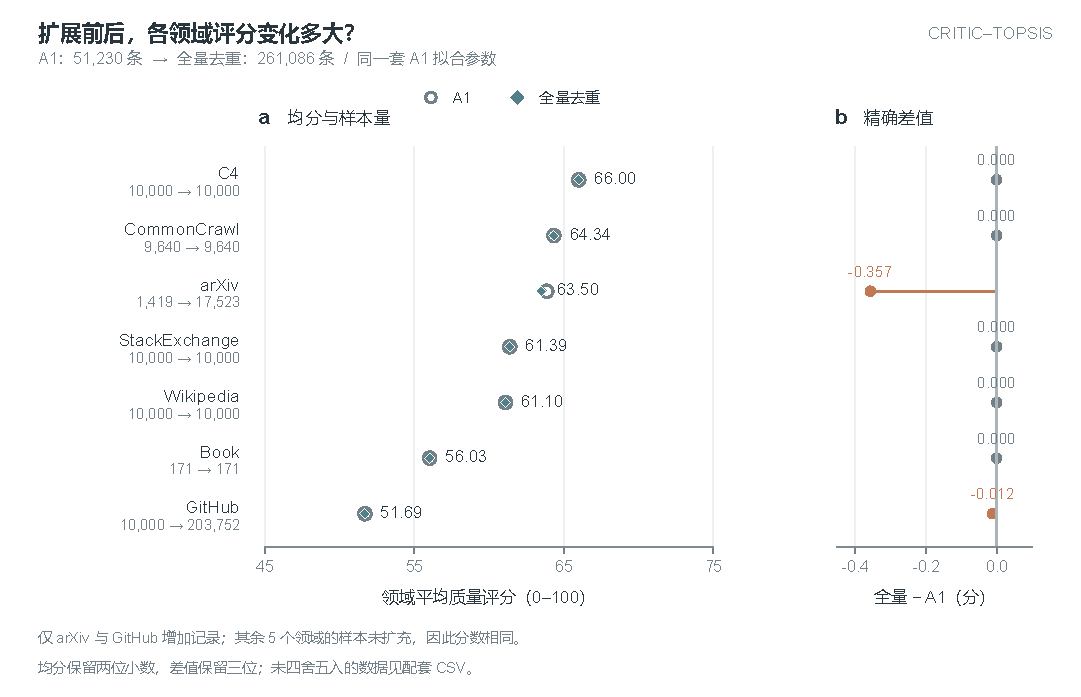
\includegraphics[width=\linewidth,height=0.42\textheight,keepaspectratio]{figures/q1-critic-topsis/nature-v1/figure03_A1_full_comparison_nature.pdf}
  \caption{领域均分对照图}
  \label{fig:q1-nature-03}
\end{figure}

\subsection{从样本级到领域级和语料级的聚合}
对领域 $g$ 的记录集合 $\mathcal{I}_g$，采用样本数加权的均值聚合。
\formulaname{领域质量均值公式}
\begin{equation}
 Q_g=\frac{1}{|\mathcal{I}_g|}\sum_{i\in\mathcal{I}_g}Q_i.
 \label{eq:q1-domain-aggregation}
\end{equation}
语料级分数同样由全体记录的样本均值给出。这种聚合保留了每条记录的等贡献原则，并能将域级差异与域规模分离：域均值反映质量，域记录数反映组成。若需降低极端值影响，可在附录中同时报告中位数和四分位距，但主结果使用均值以便与全量语料平均质量一致。
\formulaname{语料质量均值公式}
\begin{equation}
 Q_{\mathrm{corpus}}=\frac{1}{N}\sum_{i=1}^{N}Q_i.
 \label{eq:q1-corpus-aggregation}
\end{equation}

\begin{figure}[htbp]
  \centering
  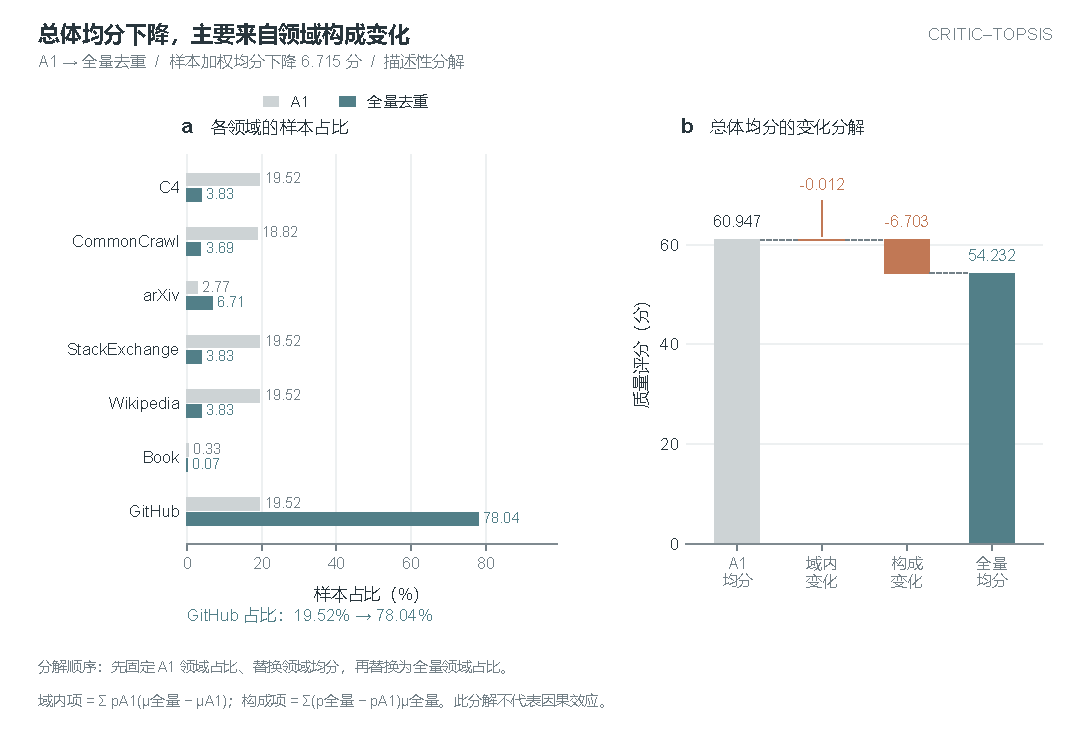
\includegraphics[width=\linewidth,height=0.42\textheight,keepaspectratio]{figures/q1-critic-topsis/nature-v1/figure04_composition_decomposition_nature.pdf}
  \caption{领域构成分解图}
  \label{fig:q1-nature-04}
\end{figure}

\subsection{全量结果与抽样集对照}
$A_1$ 语料级平均分为 $60.9471$，全量去重语料平均分为 $54.2323$，整体下降 $6.7149$ 分。按领域对照时，arxiv 从 $63.8624$ 变为 $63.5050$，下降 $0.3574$ 分；github 从 $51.7014$ 变为 $51.6893$，下降 $0.0121$ 分；book、c4、commoncrawl、stackexchange 和 wikipedia 的领域均值保持不变或仅发生四舍五入范围内的变化。由此可见，全量平均分下降主要来自领域组成变化，而不是各领域内部质量普遍恶化。GitHub 在 $A_1$ 中约占 $19.52\%$，在全量去重语料中约占 $78.04\%$，其较低的领域均值显著拉低了全量语料级分数。

\begin{table}[htbp]
  \centering
  \caption{$A_1$ 与全量去重语料的领域级质量分数对照}
  \label{tab:q1-domain-score}

  \renewcommand{\arraystretch}{1.15}
  \begin{tabular}{lrrrr}
    \toprule
    领域 & $A_1$ 均值 & 全量均值 & 变化 & 全量占比 \\
    \midrule
    arxiv & 63.8624 & 63.5050 & -0.3574 & 6.71\% \\
    book & 56.0325 & 56.0325 & 0.0000 & 0.07\% \\
    c4 & 66.0021 & 66.0021 & 0.0000 & 3.83\% \\
    commoncrawl & 64.3357 & 64.3357 & 0.0000 & 3.69\% \\
    github & 51.7014 & 51.6893 & -0.0121 & 78.04\% \\
    stackexchange & 61.3879 & 61.3879 & 0.0000 & 3.83\% \\
    wikipedia & 61.1009 & 61.1009 & 0.0000 & 3.83\% \\
    \addlinespace[0.5ex]
    语料级均值 & 60.9471 & 54.2323 & -6.7149 & 100.00\% \\
    \bottomrule
  \end{tabular}
\end{table}

\subsection{稳健性与适用边界}
将 CRITIC--TOPSIS 结果与等权加权、删除 DSIR 以及删除三个负向词组指标的敏感性方案比较。CRITIC 加权和等权结果的 Spearman 相关系数为 $0.9877$，CRITIC 结果与删除 DSIR 的结果相关系数为 $0.9860$，与删除三个负向指标的结果相关系数为 $0.9674$。在删除负向指标的方案中，平均名次变化为 $4.79$ 个百分点，约 $2.78\%$ 的记录名次变化超过 $20$ 个百分点，说明重复性指标虽不是唯一质量依据，但对尾部样本的排序具有实质影响。这里的敏感性分析用于检查第一小问质量评分对建模选择的稳定性；它不等同于问题一后续小问中对指标冲突的独立量化。

\begin{figure}[htbp]
  \centering
  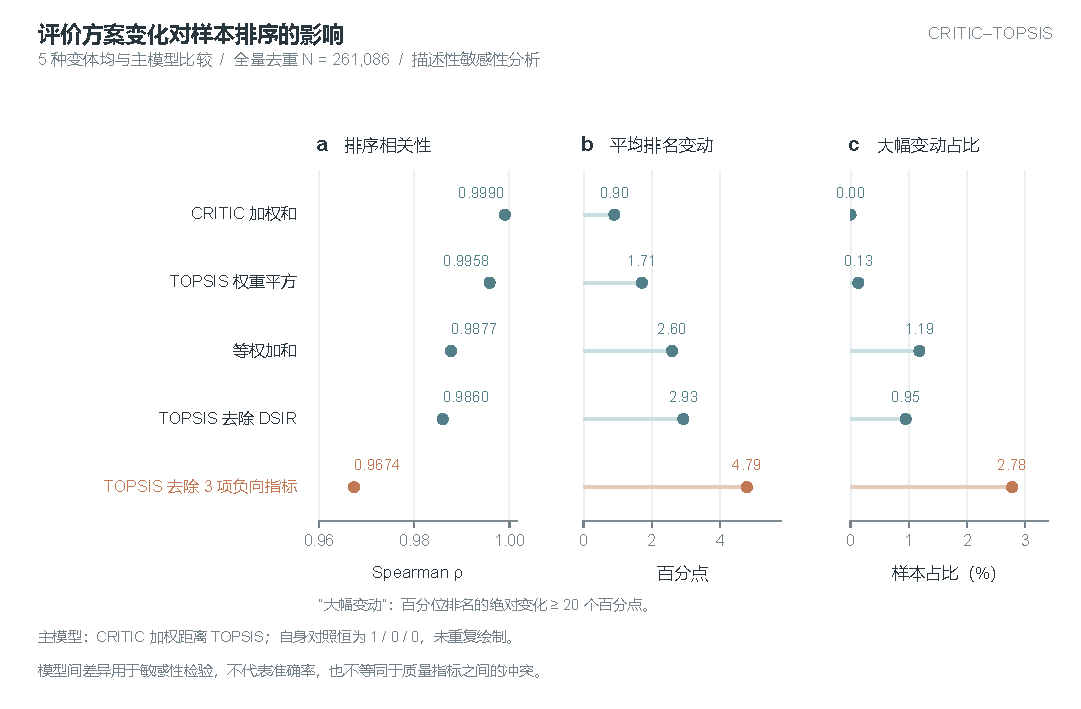
\includegraphics[width=\linewidth,height=0.42\textheight,keepaspectratio]{figures/q1-critic-topsis/nature-v1/figure06_model_sensitivity_nature.pdf}
  \caption{评分排序敏感性图}
  \label{fig:q1-nature-06}
\end{figure}

\subsection{小结}
本小问形成了一个可复算的全量质量评价链条：以 $A_1$ 的稳健边界和 CRITIC 权重建立统一标尺，以加权距离 TOPSIS 输出样本级质量分数，再按记录均值聚合为领域级和语料级分数。结果表明，$A_1$ 与扩展后的全量语料在领域内部质量上总体稳定，语料级平均分的主要变化由领域配比改变所致。该结论为后续质量冲突识别和数据配比优化提供可追溯的基线。
 引入。
%% 依照 paper/template/gmcmthesis.cls 的章节、公式、图形和 booktabs 表格规范编写。
\section{问题一：数据质量评价与基础评分}

\subsection{问题分析与总体框架}
本小问的目标是将抽样集与扩展集中的多源文本质量信号统一到同一评价尺度，形成可解释、可追溯的质量分数。评价对象包括抽样集 $A_1$、扩展集 $A_2$ 和扩展集 $A_3$ 的全部记录：$A_1$ 包含 $51{,}230$ 条记录，$A_2$ 包含 $17{,}523$ 条记录，$A_3$ 包含 $203{,}752$ 条记录。合并后先按记录指纹去重，得到 $261{,}086$ 条有效记录，去重前后删除 $11{,}419$ 条重复记录。模型流程为“全量合并与去重—指标方向统一—稳健归一化—CRITIC 客观赋权—加权距离 TOPSIS 评分—样本、领域和语料级聚合—抽样集对照”。

\begin{figure}[htbp]
  \centering
  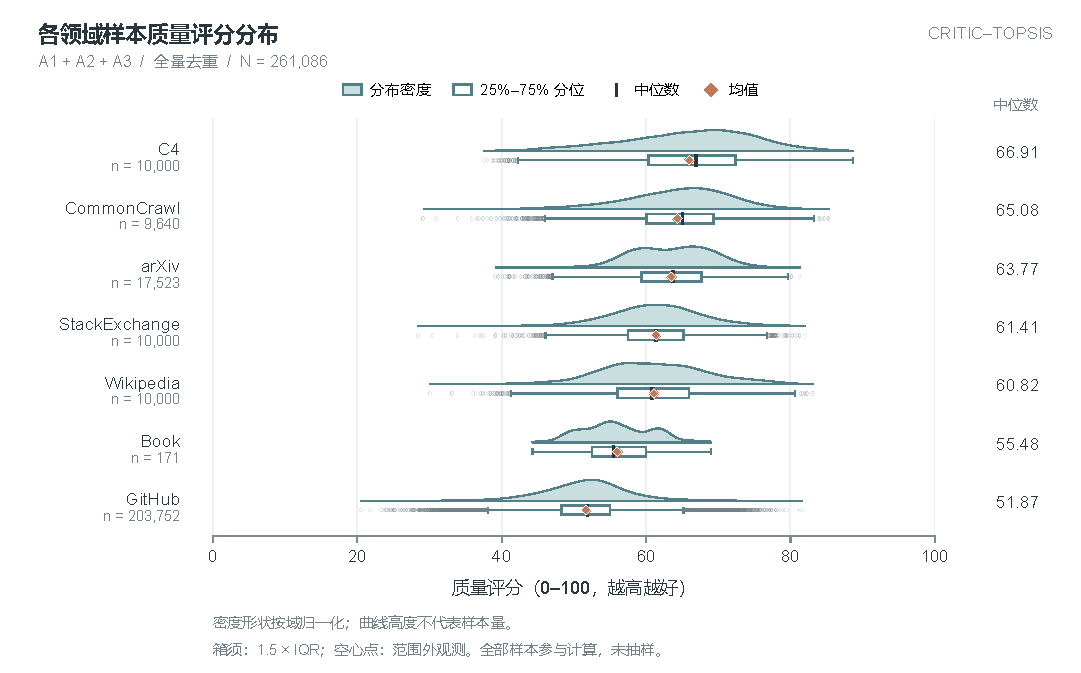
\includegraphics[width=\linewidth,height=0.42\textheight,keepaspectratio]{figures/q1-critic-topsis/nature-v1/figure01_domain_distribution_nature.pdf}
  \caption{领域质量分布图}
  \label{fig:q1-nature-01}
\end{figure}

\subsection{数据对象与预处理}
第 $i$ 条记录具有 16 维原始质量指标向量。指标覆盖语言形式、可读性、内容质量、教育性、事实性、知识覆盖与重复性等维度，其中句末标点率、cleanliness、no-ad、readability、fluency、unique words、QuRating education、writing、FineWeb education、factual、Books、Math 和 Wikipedia 为正向指标；无字母词比例、最高频二元词组占比和最高频三元词组占比为负向指标。负向指标较大时通常意味着文本更可能由符号、模板或高频短语主导，因此需要反向处理。
\formulaname{原始质量指标向量公式}
\begin{equation}
 \boldsymbol{x}_i=(x_{i1},\ldots,x_{i16}).
 \label{eq:q1-indicator-vector}
\end{equation}

正向与负向指标集合分别记为 $\mathcal P$、$\mathcal N$，两者互不相交且覆盖全部 16 个指标。方向统一后的指标定义如下。
\formulaname{指标方向统一公式}
\begin{equation}
 \widetilde{x}_{ij}=\begin{cases}
 x_{ij}, & j\in\mathcal{P},\\
 -x_{ij}, & j\in\mathcal{N}
 \end{cases}
 \label{eq:q1-direction-unification}
\end{equation}
随后使用方向统一值的 $A_1$ 拟合 $1\%$ 和 $99\%$ 分位点作为稳健边界；记边界为 $l_j$ 和 $u_j$，则统一为“越高越好”的稳健归一化形式。这里 $\operatorname{clip}(t,0,1)$ 表示将 $t$ 截断至 $[0,1]$。
\formulaname{稳健归一化公式}
\begin{equation}
 z_{ij}=\operatorname{clip}\left(\frac{\widetilde{x}_{ij}-l_j}{u_j-l_j},0,1\right).
 \label{eq:q1-robust-normalization}
\end{equation}
扩展集只使用 $A_1$ 的边界，不重新拟合分位点，从而保证 $A_1$、$A_2$ 和 $A_3$ 的分数具有可比性。归一化后检查缺失值、无穷值、越界值和重复指纹，并保留每条记录的来源集、领域标签和质量分数，供后续聚合与审计。

\begin{figure}[htbp]
  \centering
  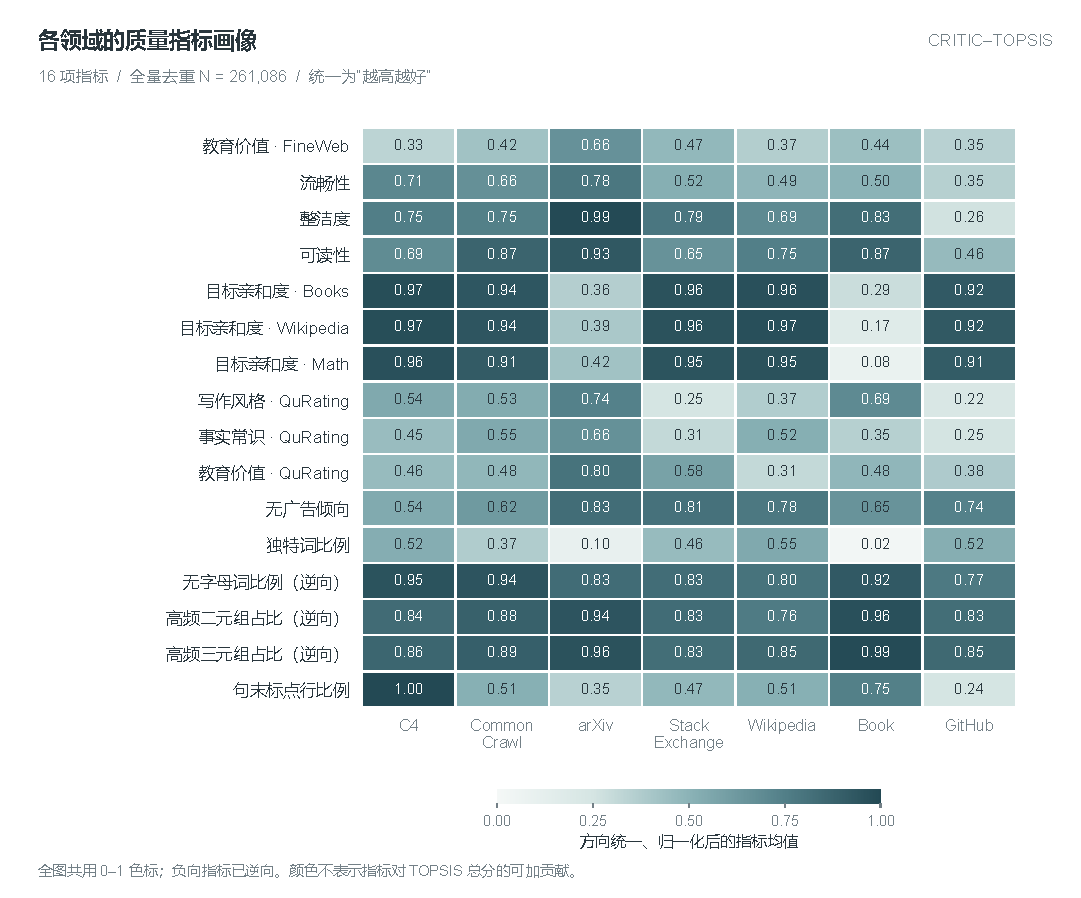
\includegraphics[width=\linewidth,height=0.42\textheight,keepaspectratio]{figures/q1-critic-topsis/nature-v1/figure02_indicator_heatmap_nature.pdf}
  \caption{领域质量指标画像图}
  \label{fig:q1-nature-02}
\end{figure}

\subsection{CRITIC 客观赋权}
为避免人为指定权重，采用 CRITIC 方法同时利用指标的离散程度和冲突程度。设归一化矩阵为 $Z$，其元素为 $z_{ij}$；第 $j$ 个指标的标准差为 $\sigma_j$，与第 $k$ 个指标的 Pearson 相关系数为 $r_{jk}$。
\formulaname{CRITIC 信息量公式}
\begin{equation}
 I_j=\sigma_j\sum_{k=1}^{16}(1-r_{jk}).
 \label{eq:q1-critic-information}
\end{equation}
\formulaname{CRITIC 权重公式}
\begin{equation}
 w_j=\frac{I_j}{\sum_{m=1}^{16}I_m}.
 \label{eq:q1-critic}
\end{equation}
其中，$\sigma_j$ 反映指标对样本的区分能力，$1-r_{jk}$ 反映该指标与其他指标的信息差异。由 $A_1$ 的拟合集计算权重并固定应用于 $A_1$ 留出集及 $A_2$、$A_3$，既防止扩展集的分布变化改变权重，又保证外推比较的可重复性。最终权重最高的指标为句末标点率（$8.9093\%$）、cleanliness（$8.0008\%$）和 no-ad（$7.7530\%$）；三个负向词组指标合计权重为 $16.5784\%$。

\begin{figure}[htbp]
  \centering
  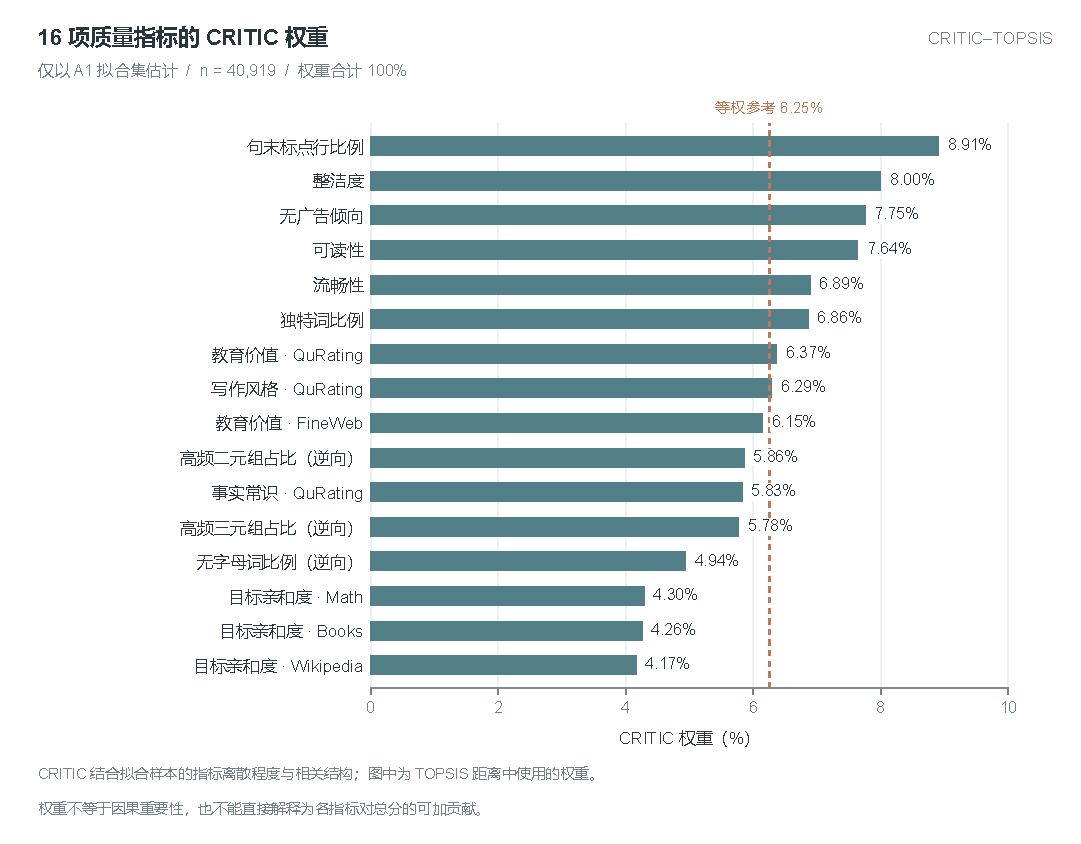
\includegraphics[width=\linewidth,height=0.42\textheight,keepaspectratio]{figures/q1-critic-topsis/nature-v1/figure05_critic_weights_nature.pdf}
  \caption{质量指标权重图}
  \label{fig:q1-nature-05}
\end{figure}

\subsection{加权距离 TOPSIS 评分}
以取值全为 1 的正向理想点 $\boldsymbol{z}^{+}$ 和取值全为 0 的负向理想点 $\boldsymbol{z}^{-}$ 为参照，计算第 $i$ 条记录到两类理想点的加权欧氏距离。
\formulaname{正理想点距离公式}
\begin{equation}
 D_i^{+}=\sqrt{\sum_{j=1}^{16}w_j(1-z_{ij})^2}.
 \label{eq:q1-topsis-positive-distance}
\end{equation}
\formulaname{负理想点距离公式}
\begin{equation}
 D_i^{-}=\sqrt{\sum_{j=1}^{16}w_jz_{ij}^2}.
 \label{eq:q1-topsis-distance}
\end{equation}
样本级质量分数定义如下，其取值在 $[0,100]$。
\formulaname{样本质量分数公式}
\begin{equation}
 Q_i=100\times\frac{D_i^{-}}{D_i^{+}+D_i^{-}}.
 \label{eq:q1-topsis-score}
\end{equation}
因此，$Q_i$ 越大表示该记录越接近理想高质量点。该分数回答的是“单条文本在 16 个统一方向质量信号下的综合质量水平”，而非某个单一指标的原始测量值。

\begin{figure}[htbp]
  \centering
  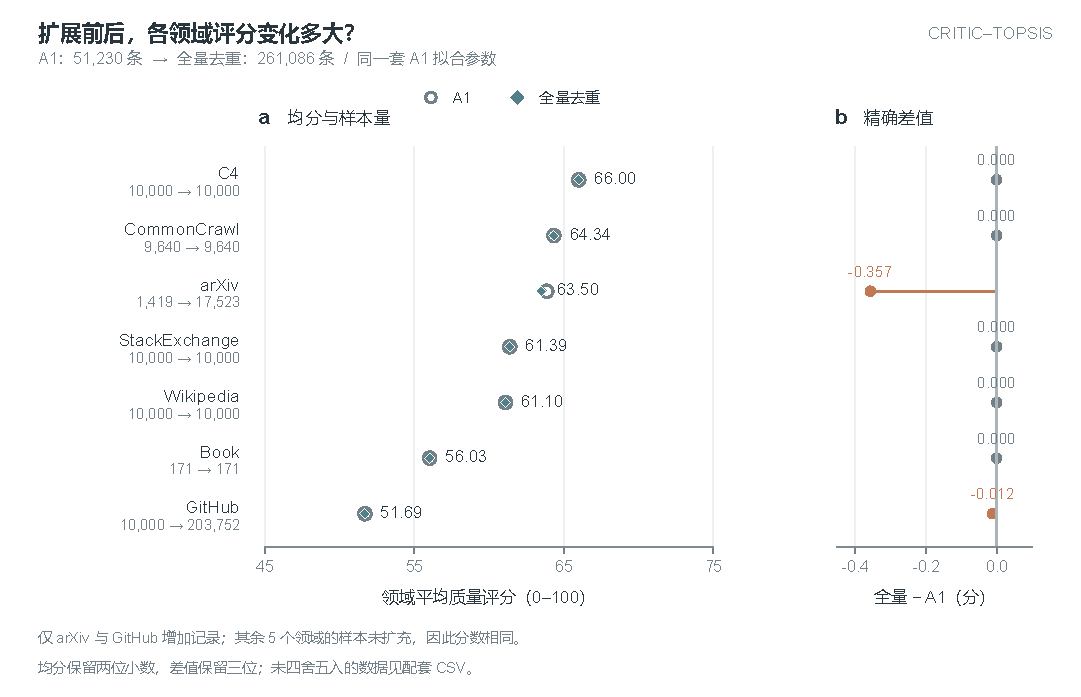
\includegraphics[width=\linewidth,height=0.42\textheight,keepaspectratio]{figures/q1-critic-topsis/nature-v1/figure03_A1_full_comparison_nature.pdf}
  \caption{领域均分对照图}
  \label{fig:q1-nature-03}
\end{figure}

\subsection{从样本级到领域级和语料级的聚合}
对领域 $g$ 的记录集合 $\mathcal{I}_g$，采用样本数加权的均值聚合。
\formulaname{领域质量均值公式}
\begin{equation}
 Q_g=\frac{1}{|\mathcal{I}_g|}\sum_{i\in\mathcal{I}_g}Q_i.
 \label{eq:q1-domain-aggregation}
\end{equation}
语料级分数同样由全体记录的样本均值给出。这种聚合保留了每条记录的等贡献原则，并能将域级差异与域规模分离：域均值反映质量，域记录数反映组成。若需降低极端值影响，可在附录中同时报告中位数和四分位距，但主结果使用均值以便与全量语料平均质量一致。
\formulaname{语料质量均值公式}
\begin{equation}
 Q_{\mathrm{corpus}}=\frac{1}{N}\sum_{i=1}^{N}Q_i.
 \label{eq:q1-corpus-aggregation}
\end{equation}

\begin{figure}[htbp]
  \centering
  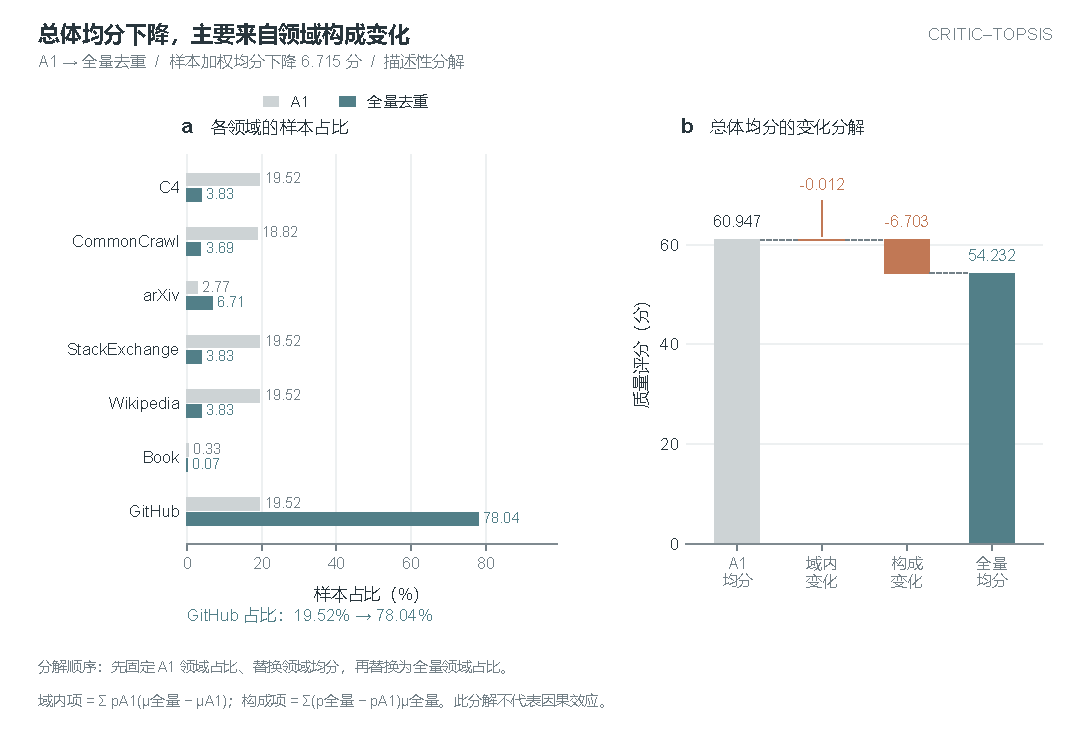
\includegraphics[width=\linewidth,height=0.42\textheight,keepaspectratio]{figures/q1-critic-topsis/nature-v1/figure04_composition_decomposition_nature.pdf}
  \caption{领域构成分解图}
  \label{fig:q1-nature-04}
\end{figure}

\subsection{全量结果与抽样集对照}
$A_1$ 语料级平均分为 $60.9471$，全量去重语料平均分为 $54.2323$，整体下降 $6.7149$ 分。按领域对照时，arxiv 从 $63.8624$ 变为 $63.5050$，下降 $0.3574$ 分；github 从 $51.7014$ 变为 $51.6893$，下降 $0.0121$ 分；book、c4、commoncrawl、stackexchange 和 wikipedia 的领域均值保持不变或仅发生四舍五入范围内的变化。由此可见，全量平均分下降主要来自领域组成变化，而不是各领域内部质量普遍恶化。GitHub 在 $A_1$ 中约占 $19.52\%$，在全量去重语料中约占 $78.04\%$，其较低的领域均值显著拉低了全量语料级分数。

\begin{table}[htbp]
  \centering
  \caption{$A_1$ 与全量去重语料的领域级质量分数对照}
  \label{tab:q1-domain-score}

  \renewcommand{\arraystretch}{1.15}
  \begin{tabular}{lrrrr}
    \toprule
    领域 & $A_1$ 均值 & 全量均值 & 变化 & 全量占比 \\
    \midrule
    arxiv & 63.8624 & 63.5050 & -0.3574 & 6.71\% \\
    book & 56.0325 & 56.0325 & 0.0000 & 0.07\% \\
    c4 & 66.0021 & 66.0021 & 0.0000 & 3.83\% \\
    commoncrawl & 64.3357 & 64.3357 & 0.0000 & 3.69\% \\
    github & 51.7014 & 51.6893 & -0.0121 & 78.04\% \\
    stackexchange & 61.3879 & 61.3879 & 0.0000 & 3.83\% \\
    wikipedia & 61.1009 & 61.1009 & 0.0000 & 3.83\% \\
    \addlinespace[0.5ex]
    语料级均值 & 60.9471 & 54.2323 & -6.7149 & 100.00\% \\
    \bottomrule
  \end{tabular}
\end{table}

\subsection{稳健性与适用边界}
将 CRITIC--TOPSIS 结果与等权加权、删除 DSIR 以及删除三个负向词组指标的敏感性方案比较。CRITIC 加权和等权结果的 Spearman 相关系数为 $0.9877$，CRITIC 结果与删除 DSIR 的结果相关系数为 $0.9860$，与删除三个负向指标的结果相关系数为 $0.9674$。在删除负向指标的方案中，平均名次变化为 $4.79$ 个百分点，约 $2.78\%$ 的记录名次变化超过 $20$ 个百分点，说明重复性指标虽不是唯一质量依据，但对尾部样本的排序具有实质影响。这里的敏感性分析用于检查第一小问质量评分对建模选择的稳定性；它不等同于问题一后续小问中对指标冲突的独立量化。

\begin{figure}[htbp]
  \centering
  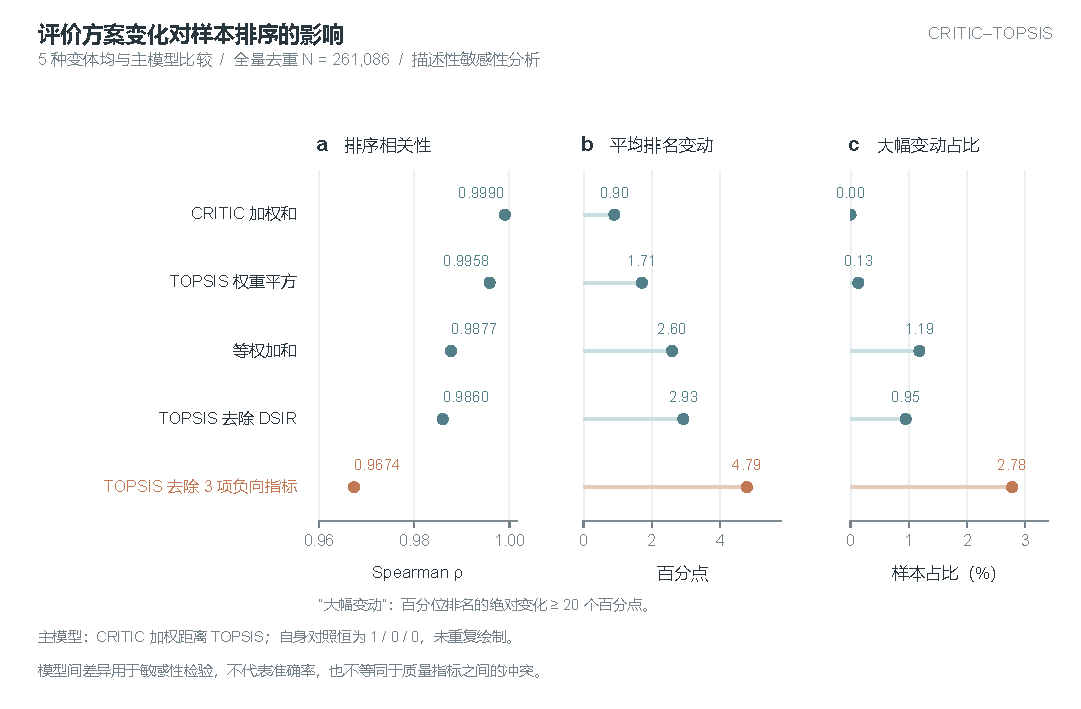
\includegraphics[width=\linewidth,height=0.42\textheight,keepaspectratio]{figures/q1-critic-topsis/nature-v1/figure06_model_sensitivity_nature.pdf}
  \caption{评分排序敏感性图}
  \label{fig:q1-nature-06}
\end{figure}

\subsection{小结}
本小问形成了一个可复算的全量质量评价链条：以 $A_1$ 的稳健边界和 CRITIC 权重建立统一标尺，以加权距离 TOPSIS 输出样本级质量分数，再按记录均值聚合为领域级和语料级分数。结果表明，$A_1$ 与扩展后的全量语料在领域内部质量上总体稳定，语料级平均分的主要变化由领域配比改变所致。该结论为后续质量冲突识别和数据配比优化提供可追溯的基线。
